\documentclass[fleqn,10pt]{wlscirep}
\usepackage[utf8]{inputenc}
\usepackage[T1]{fontenc}
\usepackage{graphics, subfigure}
%\usepackage[resetlabels, labeled]{multibib}
%\newcites{supp}{References}

\title{Machine learning topological phases in real space}

\author[1,2*]{N. L. Holanda}
\author[2,3+]{M. A. R. Griffith}
\affil[1]{Cavendish Laboratory, University of Cambridge, J. J. Thomson Avenue, Cambridge, CB3 0HE, United Kingdom}
\affil[2]{Centro Brasileiro de Pesquisas F\'isicas, Rua Dr. Xavier Sigaud, 150, Urca, 22290-180,  Rio de Janeiro, RJ, Brazil}
\affil[3]{Departamento de Ciências Naturais, Universidade Federal de S\~ao Jo\~ao Del Rei, Praça Dom Helv\'ecio 74, 36301-160, S\~ao Jo\~ao Del Rei, MG, Brazil}


\affil[*]{linneuholanda@gmail.com, linneu@cbpf.br}

\affil[+]{griffithphys@gmail.com}

\begin{abstract}
We develop a supervised machine learning algorithm that is able to learn topological phases for finite condensed matter systems from bulk data in real lattice space. The algorithm employs diagonalization in real space together with any supervised learning algorithm to learn topological phases through an eigenvector ensembling procedure. We combine our algorithm with decision trees and random forests to successfully recover topological phase diagrams of Su-Schrieffer-Heeger (SSH) models from bulk lattice data in real space and show how the Shannon information entropy of ensembles of lattice eigenvectors can be used to retrieve a signal detailing how topological information is distributed in the bulk. The discovery of Shannon information entropy signals associated with topological phase transitions from the analysis of data from several thousand SSH systems illustrates how model explainability in machine learning can advance the research of exotic quantum materials with properties that may power future technological applications such as qubit engineering for quantum computing. 
\end{abstract}
\begin{document}
\nocite{*}

\flushbottom
\maketitle
% * <john.hammersley@gmail.com> 2015-02-09T12:07:31.197Z:
%
%  Click the title above to edit the author information and abstract
%
\thispagestyle{empty}

%\noindent Please note: Abbreviations should be introduced at the first mention in the main text – no abbreviations lists. Suggested structure of main text (not enforced) is provided below.

\section*{Introduction}

The quest for innovative materials that harness exotic quantum properties has lured physicists into the realm of topological insulators and topological states of matter \cite{RevModPhys.82.3045}. These materials feature previously unthought-of traits like bulk insulation coupled with metallic conductance at the surface and the splitting of currents according to spin orientation. Adding to that, these properties are protected by non-trivial topology that renders them robust to many sources of perturbation like thermal noise. Such characteristics make them promising candidates to being the cornerstone of 21st century technologies like spintronics and quantum computing.

These new topological states of matter have been studied in several contexts in condensed matter physics including superconductors \cite {CONTINENTINO2017A1}$^-$\cite{ryu2010topological}, ultracold atoms \cite{atala2013direct}$^-$\cite{meier2016observation}, photonic crystals \cite{hafezi2013imaging}$^-$\cite{PhysRevX.5.031011}, photonic quantum walks \cite{kitagawa2012observation}$^-$\cite{PhysRevX.7.031023} and Weyl semimetals \cite{soluyanov2015type,PhysRevX.5.031013}. Among these, the Su-Schrieffer-Heeger (SSH) model \cite{PhysRevLett.42.1698} has attracted particular theoretical interest due to its simplicity and generality.

The SSH model is the simplest tight-binding model that exhibits a topological phase transition. As such, it can be viewed as the \emph{Drosophila} of the field, providing a simple framework for testing new techniques. The model can be expressed in terms of creation and annihilation operators by the Hamiltonian
\begin{equation}
\label{SSH_ham}
\hat{H}(\mathbf{t})=\mathbf{c}^{\dagger}H(\mathbf{t})\mathbf{c}
\end{equation}
and describes e.g. the hopping of electrons along a one-dimensional chain comprising two atoms per unit cell (a brief discussion of the SSH model and its topological properties can be found in the section \textbf{The SSH model} in the Supplementary Material). The SSH model has found several interesting applications in the modelling of diverse systems with non-trivial topology like optical lattices \cite{maffei2018topological}, polymeric materials \cite{RevModPhys.73.681} and topological mechanisms \cite{kane2014topological,Chen13004}.

Many recent papers have explored the possibility of treating the general problem of determining phase transition boundaries of physical systems as machine learning tasks \cite{carrasquilla2017machine}$^-$\cite{rodriguez2018identifying}. In the particular case of topological phase transitions, the usual approach for supervised learning is to generate a data set $\big(H_1(k), W_1\big)$, ..., $\big(H_n(k), W_n\big)$ whose inputs are representations of Hamiltonians in wavevector space $H_i(k)$ and targets are their corresponding topological invariants $W_i$ (for the SSH model the topological invariant is the winding number). Our paper extends this task to the case of learning topological phase diagrams from input data in real space. Strikingly, we find that information localized on a few lattice sites in the bulk is sufficient to predict with high accuracy which topological phase a particular Hamiltonian belongs to.

To investigate topological phases of matter in real space we have designed a novel supervised learning algorithm (here called eigenvector ensembling algorithm) tailored for the task of learning phase transition boundaries from local features. The algorithm is based on eigenvector decomposition and eigenvector ensembling and therefore will require minimal changes to be applicable to a broader class of data-driven physics problems. We demonstrate its effectiveness by combining it with decision trees and random forests to recover the topological phase diagrams of SSH systems from local coordinates of eigenstates in real space.

The advantage of using decision tree-based algorithms to learn topological phases from local eigenvector data is that their use of entropy-based cost functions (such as Shannon information entropy or Gini impurity) furnishes them with an intrinsinc model explanaibility tool that summarizes how important each feature was to learn the desired pattern in the data. This makes it much easier to trace the localization of relevant information along the features of a data set. Here we use the Shannon information entropy of ensembles of real space eigenvectors to recover a signal quantifying the amount of topological information available from each lattice site. This is a highly non-trivial proposition since the topological phase of a system is a global property of the whole system emerging from complex interactions between its components, and therefore even defining a local topological signal is a daunting theoretical task. To our knowledge this is the first time that a signal describing the localization of topological information in the bulk of topological condensed matter systems is presented in the literature.

The Shannon information entropy signals presented for the first time in this work provide a clear illustration of how model explainability in machine learning can guide new discoveries in condensed matter and quantum materials physics, since the existence of these signals was established by analyzing data from several thousand SSH systems which, taken individually, could not have provided any concrete hint of their existence. 

\begin{figure}
\centering
\subfigure[]{\label{ssh1}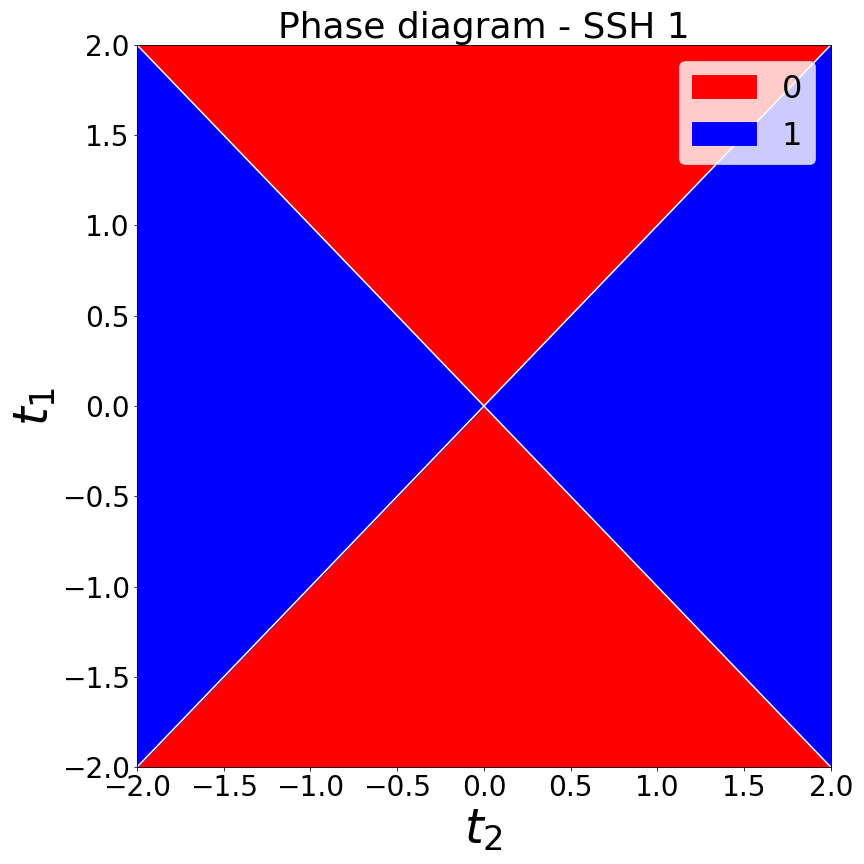
\includegraphics[width=.45\textwidth]{./phase_diagrams/ssh1.png}}\quad
\subfigure[]{\label{ssh2}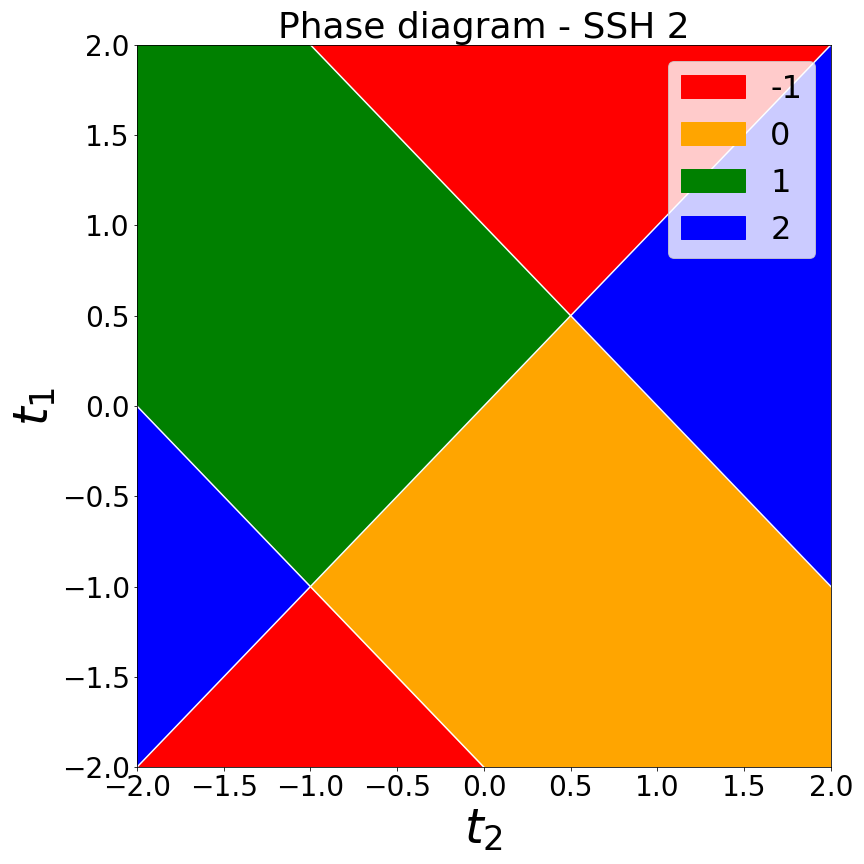
\includegraphics[width=.45\textwidth]{./phase_diagrams/ssh2.png}}
\caption{Phase diagrams in parameter space. a) SSH model with first-neighbor hoppings $t_1$ and $t_2$. The (red) regions with winding number $W$ = 0 are trivial, while the (blue) regions with winding number $W$ = 1 are topologically non-trivial. b) SSH model with first ($t_1$ and $t_2$) and second ($T_1$ and $T_2$) nearest-neighbor hoppings. In this article we set $t_1$ = $t_2$ = 1 and renamed the variables $T_1$ $\rightarrow$ $t_1$, $T_2$ $\rightarrow$ $t_2$ for convenience. The (orange) region with winding number $W$ = 0 is trivial while the others with winding numbers $W$ = -1, $W$ = 1 and $W$ = 2 (red, green and blue respectively) are topologically non-trivial.}
\label{fig:phasediagrams}
\end{figure}

\section*{Numerical experiments}

The eigenvector ensembling algorithm consists of five steps: 1) Generating Hamiltonians in real space and their corresponding winding numbers; 2) Creating training, validation and test sets; 3) Training on real space eigenvectors of Hamiltonians in the training set; 4) Eigenvector ensembling and 5) Bootstrapping. A detailed description of the algorithm is found in the section \textbf{The eigenvector ensembling algorithm} in the Supplementary Material. Here we present results of the numerical experiments we performed with it. We start with the results from the simplest case, the SSH model with nearest-neighbor hopping (here called SSH 1, figure \ref{ssh1}), then we analize the SSH model with first and second nearest-neighbor hoppings (here called SSH 2, figure \ref{ssh2}).

In each experiment our grid consisted of 6561 Hamiltonians uniformly distributed in the closed square $[-2,2]\times[-2,2]$ in the $t_1$-$t_2$ plane in parameter space. The goal in each experiment is to recover the corresponding phase diagram in 2D (two-dimensional) parameter space, figures \ref{ssh1} and \ref{ssh2}, from local lattice data in the much higher-dimensional real space (100D - in both experiments lattices have 50 unit cells, yielding 100$\times$100 Hamiltonian matrices).

This task is particularly hard near phase transition boundaries, where numerical computation of winding numbers become less stable. For this reason, when sampling the training set we only consider those Hamiltonians in the grid whose numerically computed winding numbers lie in a range $\epsilon = 0.01$ around the allowed winding number values. Therefore, a good performance metric is the accuracy measured at those Hamiltonians near phase transitions that are never used for training, and thus we assign them to the test set. The remaining Hamiltonians in the grid are split into training and validation sets as detailed in the subsections below.

When generating the Hamiltonians we applied periodic boundary conditions to eliminate border effects. This should make recovering a topological signal from local eigenvector coordinates even harder, since in this case the translational symmetry of the systems should allow for no obvious way to distinguish between unit cells. The choice of periodic boundary conditions also implies that the information recovered from real space data comes from the bulk of the topological systems considered and therefore provides strong evidence for the existence of topological signatures in the bulk of such systems. 

Figures \ref{figexp1_exp} and \ref{figexp2_exp} respectively illustrate single iterations of experiments 1 and 2 as seen from parameter space. The accuracy statistics presented in the following subsections and probability heatmaps shown in figures \ref{ssh1_heatmaps} and \ref{ssh2_heatmaps} were obtained after bootstrapping each experiment $n_{exp}$ = 100 times. The recovered probability heatmaps faithfully portray the phase diagrams in figure \ref{fig:phasediagrams}, with clear phase transition lines appearing in the regions of highest uncertainty.

\subsection*{Experiment 1: Learning a first-neighbor hopping SSH model with decision trees}

Our test set in this experiment contained 1005 Hamiltonians (approx. 15.3\% of all data). Of the remaining 5556 Hamiltonians, 556 were randomly assigned to the training set (approx. 8.5\%) and 5000 (approx. 76.2\%) were used to compute validation scores at each iteration. These proportions between training and validation sets are such that approximately 10\%  of Hamiltonians from outside of the test set were used for training at each iteration. The composition of the train + validation set for this experiment was 50.8\% of Hamiltonians with winding number $W$ = 0 and 49.2\% with winding number $W$ = 1. The composition of the test set was 44.8\% of Hamiltonians with winding number $W$ = 0 and 55.2\% with winding number $W=1$. Our algorithm of choice for this experiment was a simple decision tree model \cite{breiman2017classification}.

The bootstrap allows us to collect several statistics to evaluate performance. In particular, we report mean accuracies on training eigenvectors (98.2\%), validation eigenvectors (96.4\%) and test eigenvectors (78.8\%). Eigenvector ensembling substantially improved mean accuracies for Hamiltonians. These were 100\% for training Hamiltonians, 100\% for validation Hamiltonians and 99.1\% for test Hamiltonians.

The probability heatmaps and phase diagram learned by the combination of decision trees with eigenvector ensembling used in experiment 1 are shown in figure \ref{ssh1_heatmaps}.

\begin{figure}
\centering
\subfigure[]{\label{figexp1_exp:a}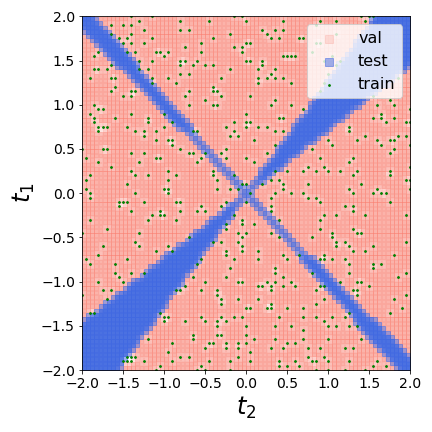
\includegraphics[width=.32\textwidth]{./ssh1/periodic_100_6561/scatter_train_val_test_experiment_0.png}}\quad
\subfigure[]{\label{figexp1_exp:b}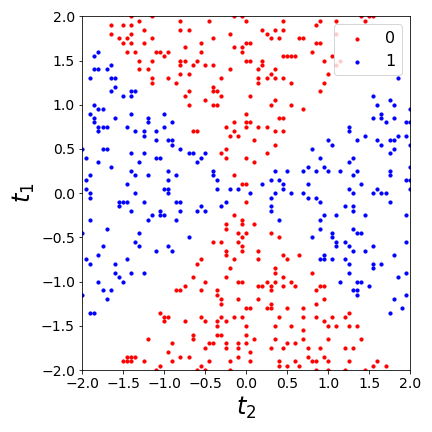
\includegraphics[width=.32\textwidth]{./ssh1/periodic_100_6561/scatter_winding_train_experiment_0.png}}
\subfigure[]{\label{figexp1_exp:c}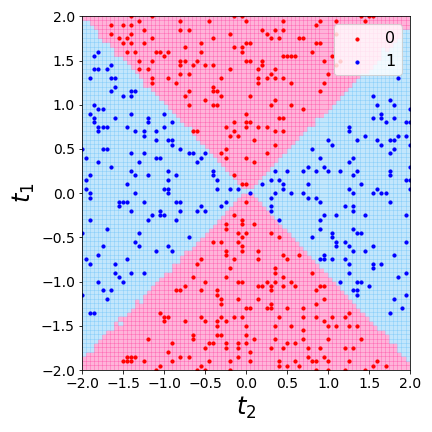
\includegraphics[width=.32\textwidth]{./ssh1/periodic_100_6561/pcolormesh_prediction_grid_experiment_0.png}}
\caption{Visualization of a single iteration of experiment 1 as seen from 2D parameter space. (a) Train/validation/test split. (b) Distribution of winding numbers in the training set. (c) Phase diagram learned from real space lattice data by a combination of decision tree and eigenvector ensembling.}
\label{figexp1_exp}
\end{figure}

\subsection*{Experiment 2: Learning a first- and second-neighbor hoppings SSH model with random forests}
\label{exp2}

This task is considerably more difficult than the previous one due to the higher number of classes and the fact that some of the labels encompass disconnected regions. For this reason, instead of using a single decision tree, we upgraded our model to a random forest \cite{Breiman2001} with 25 decision trees. Our data set consisted of 1040 (15.8\%) test Hamiltonians. The remaining Hamiltonians are randomly split in half between training and validation sets at each iteration, giving 2761 (42.1\%) training Hamiltonians and 2760 (42.1\%) validation Hamiltonians. The distribution of winding numbers for the Hamiltonians in the train + validation set for this experiment was $W$ = -1 (17.9\%), $W$ = 0 (32.5\%), $W$ = 1 (32.3\%) and $W$ = 2 (17.3\%). The distribution of winding numbers for the Hamiltonians in the test set was $W$ = -1 (36.3\%), $W$ = 0 (11.1\%), $W$ = 1 (12.7\%) and $W$ = 2 (39.9\%).

Mean accuracies across 100 repetitions of experiment 2 were 99.9\% for training eigenvectors, 97.1\% for validation eigenvectors and 66.4\% for test eigenvectors. Mean accuracies resulting from eigenvector ensembling were 100\% for training Hamiltonians, 99.7\% for validation Hamiltonians and 88.2\% for test Hamiltonians. The large accuracy gain achieved by eigenvector ensembling in the test set (going from 66.4\% eigenvector accuracy to 88.2\% Hamiltonian accuracy) attests to its power.

The probability heatmaps and phase diagram learned by the combination of random forests with eigenvector ensembling used in experiment 2 are shown in figure \ref{ssh2_heatmaps}.

\begin{figure}
\centering
\subfigure[]{\label{figexp2_exp:a}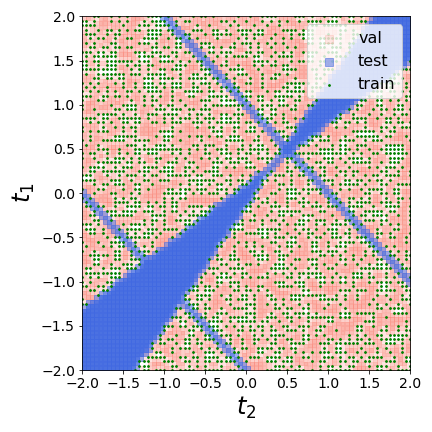
\includegraphics[width=.32\textwidth]{./ssh2/periodic_100_6561/scatter_train_val_test_experiment_0.png}}\quad
\subfigure[]{\label{figexp2_exp:b}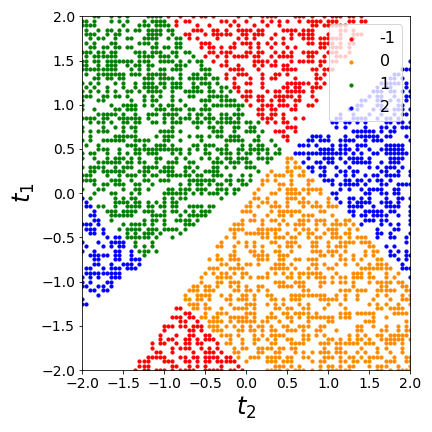
\includegraphics[width=.32\textwidth]{./ssh2/periodic_100_6561/scatter_winding_train_experiment_0.png}}
\subfigure[]{\label{figexp2_exp:c}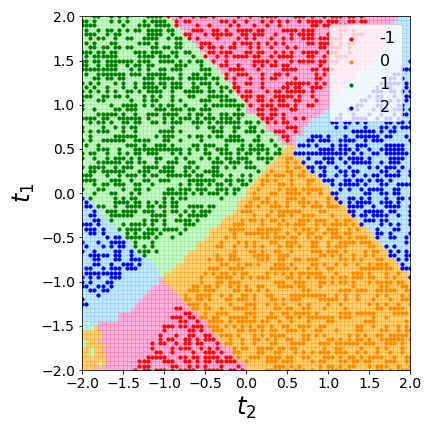
\includegraphics[width=.32\textwidth]{./ssh2/periodic_100_6561/pcolormesh_prediction_grid_experiment_0.png}}
\caption{Visualization of a single iteration of experiment 2 as seen from 2D parameter space. (a) Train/validation/test split. (b) Distribution of winding numbers in the training set. (c) Phase diagram learned from real space lattice data by a combination of random forest and eigenvector ensembling.}
\label{figexp2_exp}
\end{figure}

\section*{Information entropy signatures}

We now analyze how the algorithm was able to recover a global property of the Hamiltonians (their topological phase) from bulk local features (real space eigenvector coordinates on each lattice site). Alongside the fact that decision trees and random forests are very easy to train and visualize, the other reason that led us to test our algorithm with them was that they allow us to check which features (and thus which lattice sites) were most informative in training.

The (normalized) relevance of a feature is given by how much it reduces a loss function (e.g. Shannon information entropy or Gini impurity \cite{friedman2001elements}). By averaging normalized relevances as measured by reduction in the information entropy of ensembles of real space eigenvectors across $n_{exp}$ = 100 iterations of both experiment 1 and experiment 2 we recovered Shannon entropy signals that reveal which lattice sites were consistently more relevant in learning topological phases from data in real space for each experiment. These signals are the information entropy signatures of each topological phase transition. 

The bar plots in figure \ref{feature_importances} show how informative each lattice site was in learning topological phases for experiments 1 and 2. They represent the information entropy signatures along the lattices in each SSH system. For experiment 1, only six lattice sites $S_1$ = (0, 1, 3, 50, 51, 53) corresponding to the two sharp peaks seen in figure \ref{feature_importances_ssh1} contributed approximately 70\% of total reduction in Shannon entropy. Similarly, approximately 30\% of total reduction in the Shannon information entropy of eigenvector data from experiment 2 was achieved by eighteen lattice sites $S_2$ = (0, 1, 2, 3, 4, 5, 46, 48, 49, 50, 51, 53, 94, 95, 96, 97, 98, 99) distributed along the three peaks in figure \ref{feature_importances_ssh2}.

Each of the information entropy signatures shown in figure \ref{feature_importances} captures a general pattern that persists regardless of the length of the lattice (i.e, number of unit cells) used to compute them. They are not, therefore, artifacts of particular choices of hyperparameters used to run the eigenvector ensembling algorithm. We present the information entropy signatures for longer lattices in the section \textbf{Information entropy signatures in the macroscopic limit} in the Supplementary Material.

To see if learning the topological phases can be achieved efficiently by employing simpler models we reran experiments 1 and 2 using only a small subset of most relevant lattice sites. In our rerun of experiment 1 using only lattice sites $S'_1$ = (0, 50, 51, 99) (which contributed approximately 45 \% of total reduction in Shannon information entropy in experiment 1), mean accuracies were 97.0\% for training eigenvectors, 91.5\% for validation eigenvectors and 72.8\% for test eigenvectors. Mean accuracies obtained from eigenvector ensembling were 99.1\% for training Hamiltonians, 99.5\% for validation Hamiltonians and 94.5\% for test Hamiltonians.

Mean accuracies for our rerun of experiment 2 using only lattice sites $S'_2$ = (0, 1, 3, 48, 50, 51, 96, 98, 99) (which contributed approximately 20 \% of total reduction in Shannon information entropy in experiment 2) were 99.9\% for training eigenvectors, 87.7\% for validation eigenvectors and 47.3\% for test eigenvectors. Eigenvector ensembling yields mean accuracies of 100\% for training Hamiltonians, 99.5\% for validation Hamiltonians and 74.5\% for test Hamiltonians.  

These results demonstrate that learning topological phases from local real space data in the bulk is still possible even for small subsets of lattice sites. We refer the reader to the section \textbf{Learning topological phases from real space data} in the Supplementary Material for a discussion of how this is possible.

\begin{figure}
\centering
\subfigure[]{\label{ssh1_heatmap_0}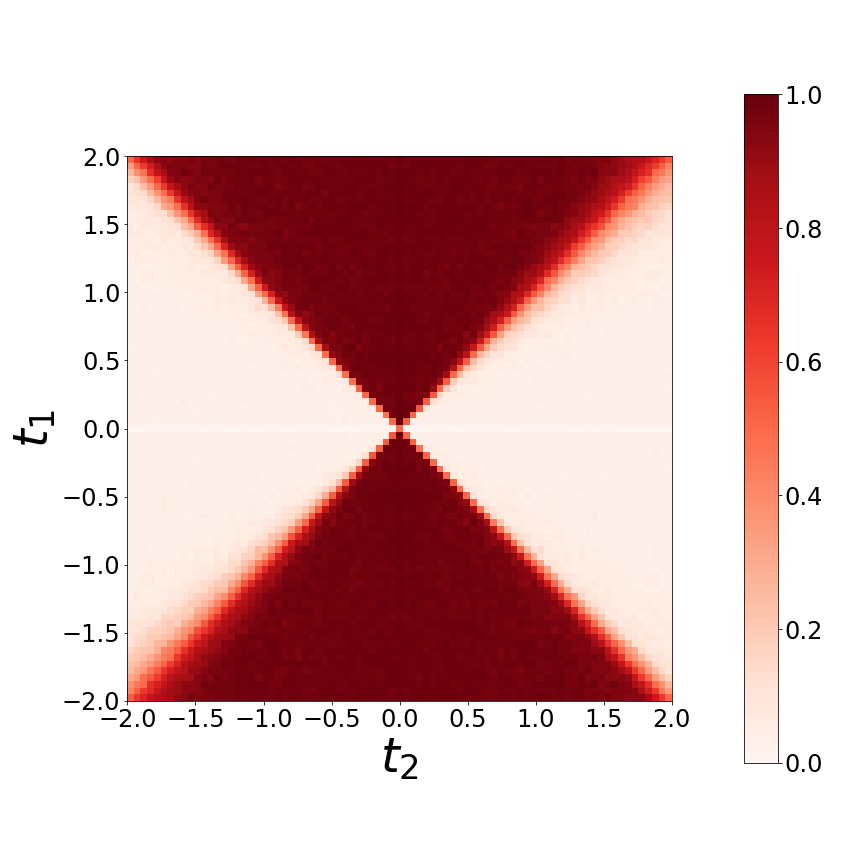
\includegraphics[width=.32\textwidth]{./ssh1/periodic_100_6561/imshow_winding_grid_winding_0_sim.png}}
\subfigure[]{\label{ssh1_heatmap_1}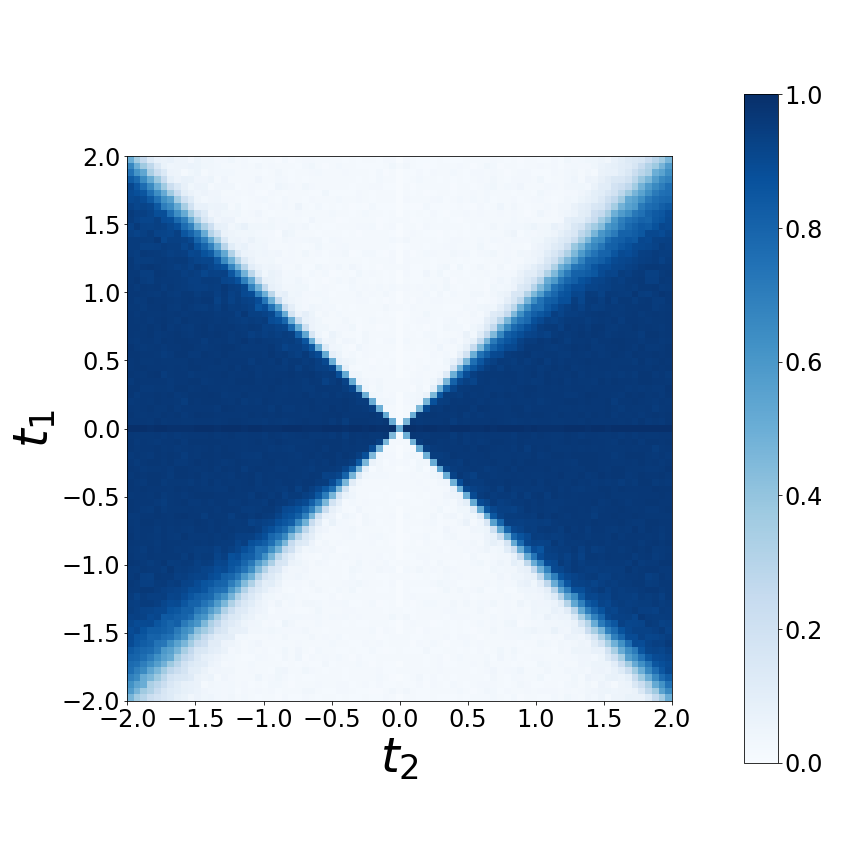
\includegraphics[width=.32\textwidth]{./ssh1/periodic_100_6561/imshow_winding_grid_winding_1_sim.png}}
\subfigure[]{\label{ssh1_heatmap}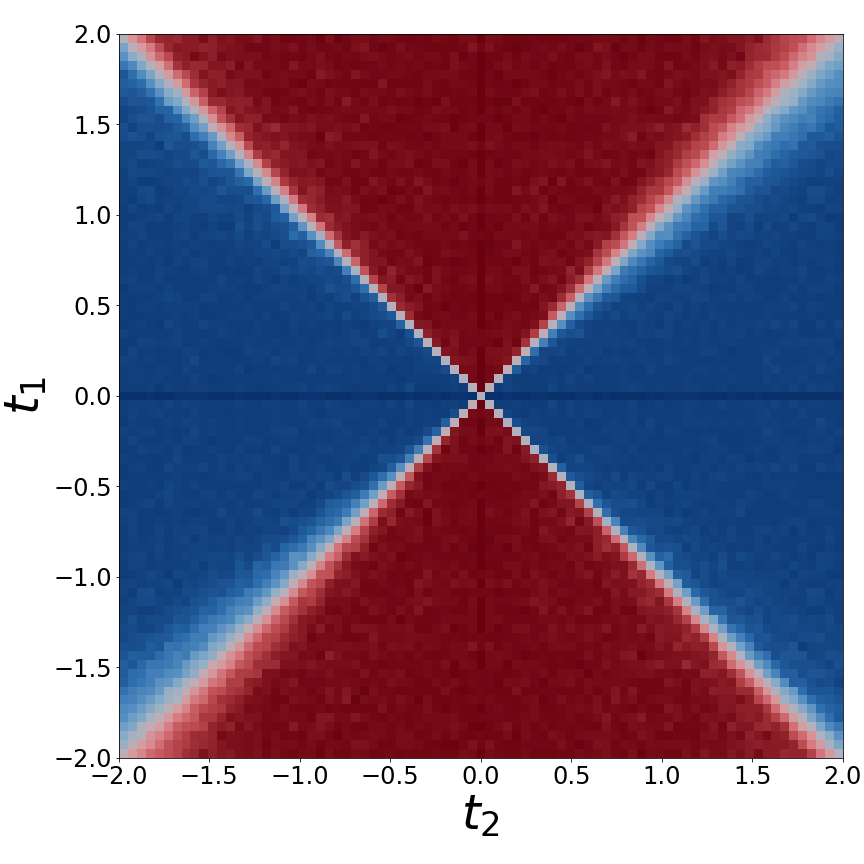
\includegraphics[width=.32\textwidth]{./ssh1/periodic_100_6561/merge_imshow_winding_grids_second_sim.png}}
\caption{Probability heatmaps learned by a combination of decision trees with eigenvector ensembling from bulk real space eigenvector data in experiment 1. Heatmaps were averaged across all 100 iterations of the experiment. (a) Probability heatmap showing the probability that a Hamiltonian in the grid has winding number equal to 0.  (b) Probability heatmap showing the probability that a Hamiltonian in the grid has winding number equal to 1. (c) The phase diagram resulting from heatmaps (a) and (b).}
\label{ssh1_heatmaps}
\end{figure}

\begin{figure}
\centering
\subfigure[]{\label{ssh2_heatmap_-1}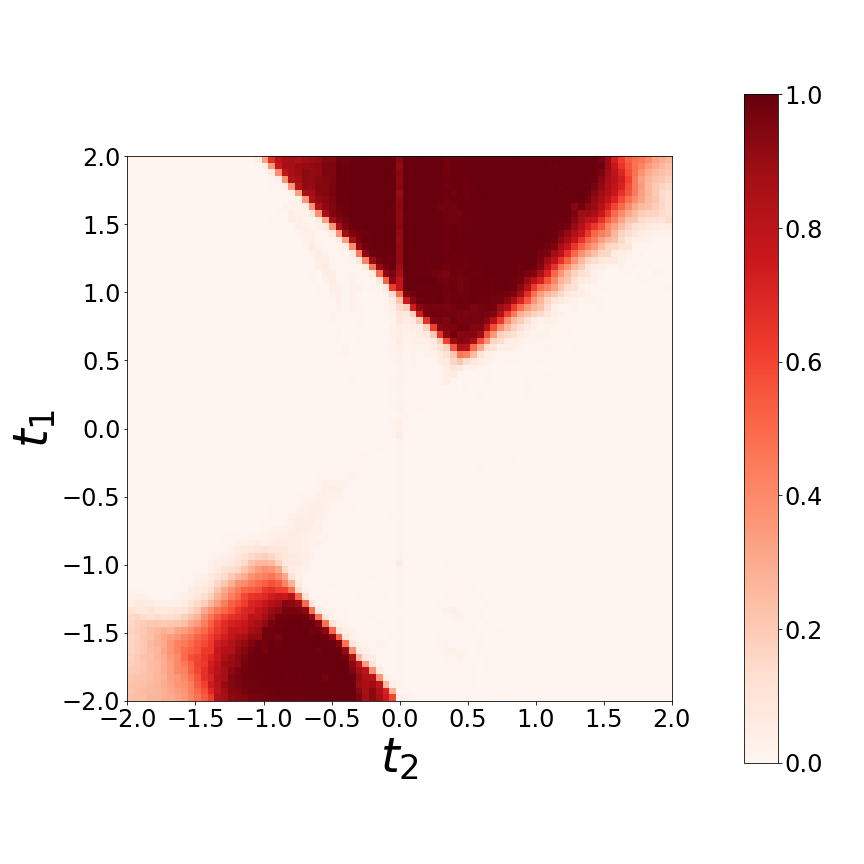
\includegraphics[width=.32\textwidth]{./ssh2/periodic_100_6561/imshow_winding_grid_winding_-1_sim.png}}
\subfigure[]{\label{ssh2_heatmap_0}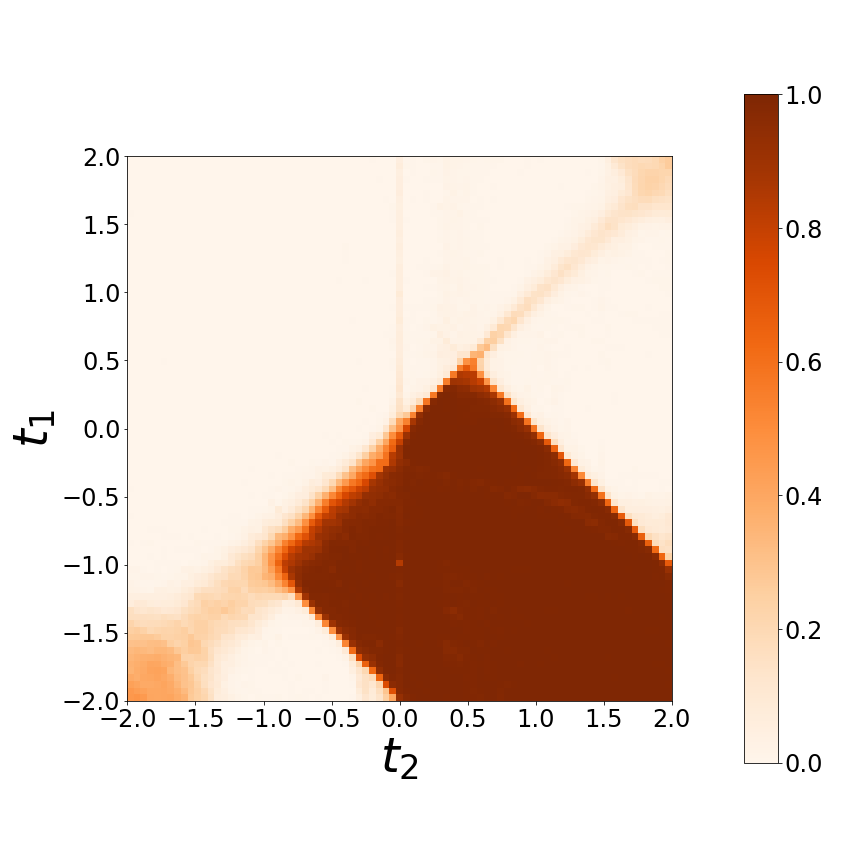
\includegraphics[width=.32\textwidth]{./ssh2/periodic_100_6561/imshow_winding_grid_winding_0_sim.png}}
\subfigure[]{\label{ssh2_heatmap_1}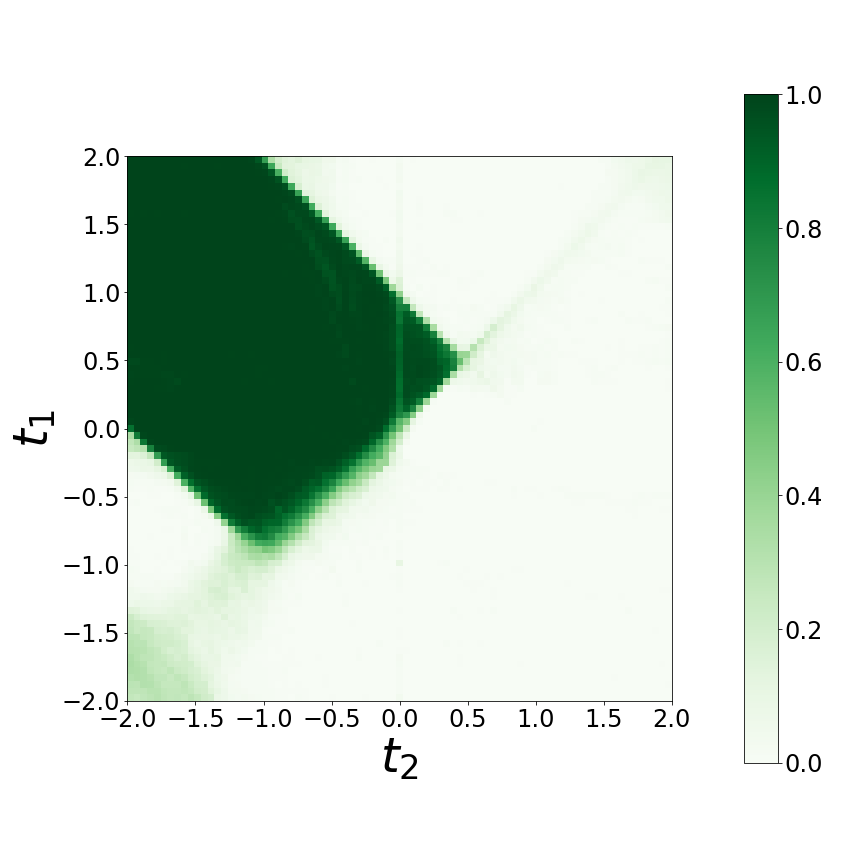
\includegraphics[width=.32\textwidth]{./ssh2/periodic_100_6561/imshow_winding_grid_winding_1_sim.png}}
\subfigure[]{\label{ssh2_heatmap_2}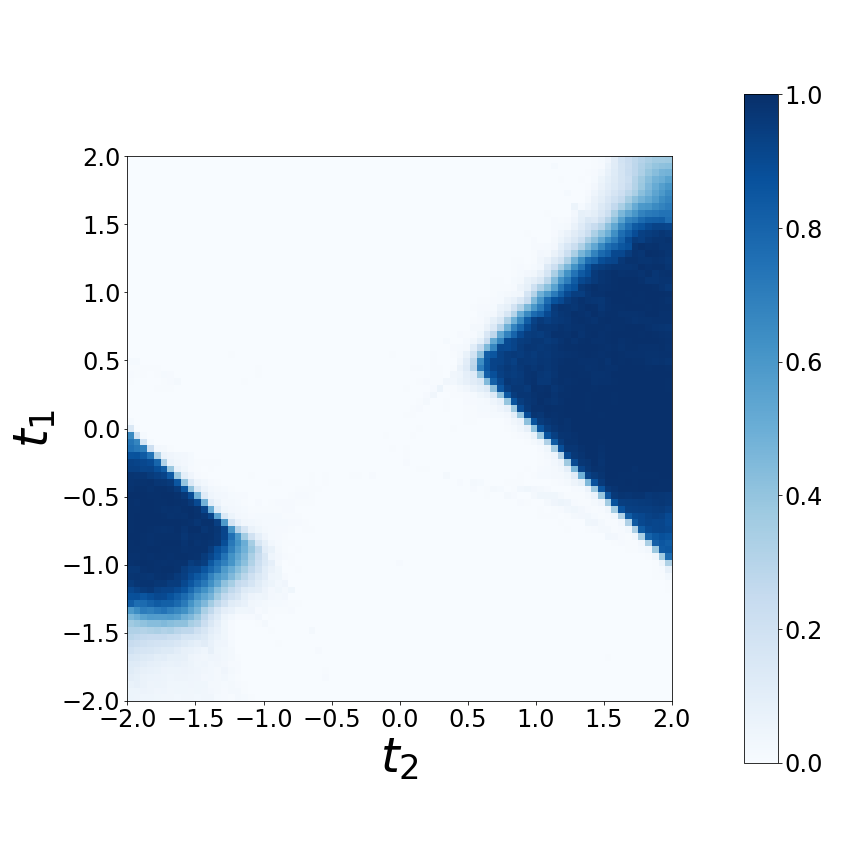
\includegraphics[width=.32\textwidth]{./ssh2/periodic_100_6561/imshow_winding_grid_winding_2_sim.png}}
\subfigure[]{\label{ssh2_heatmap}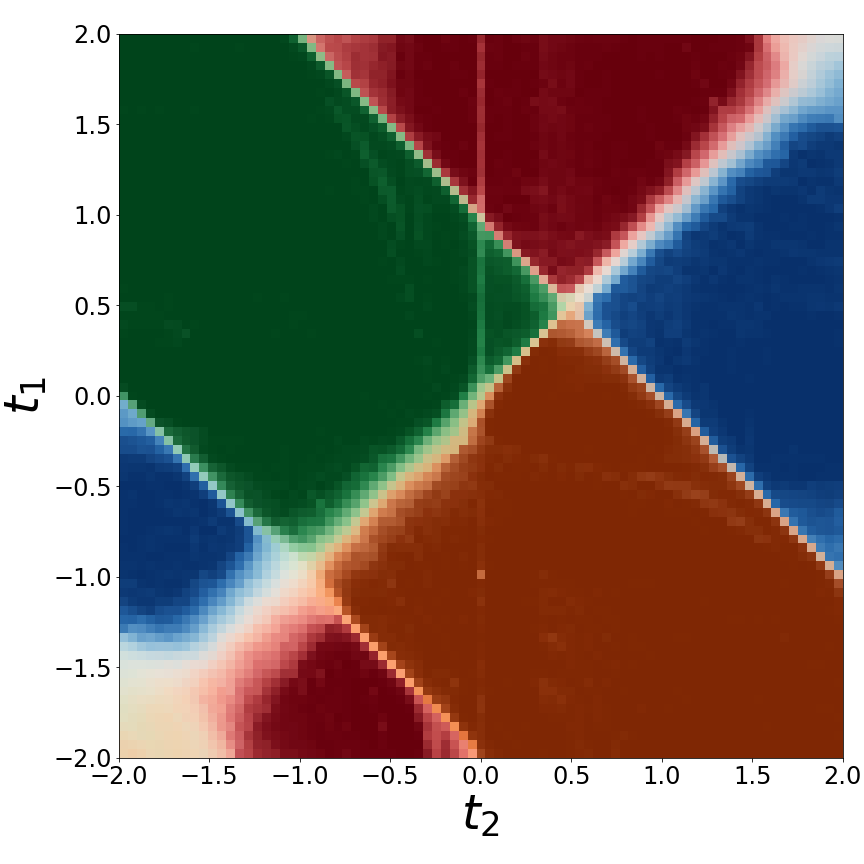
\includegraphics[width=.32\textwidth]{./ssh2/periodic_100_6561/merge_imshow_winding_grids_sim.png}}
\caption{Probability heatmaps learned by a combination of random forests with eigenvector ensembling from bulk real space eigenvector data in experiment 2. Heatmaps were averaged across all 100 iterations of the experiment. (a) Probability heatmap showing the probability that a Hamiltonian in the grid has winding number equal to -1.  (b) Probability heatmap showing the probability that a Hamiltonian in the grid has winding number equal to 0. (c) Probability heatmap showing the probability that a Hamiltonian in the grid has winding number equal to 1. (d) Probability heatmap showing the probability that a Hamiltonian in the grid has winding number equal to 2. (e) The phase diagram resulting from heatmaps (a)-(d).}
\label{ssh2_heatmaps}
\end{figure}

\section*{Discussion}

Given the increasing complexity of systems studied in condensed matter physics and the rising demand for materials with exotic and robust properties to power future technological progress, it is only expected that data-driven approaches to physics will grow in demand. Our work represents a step in this direction, as we have implemented a data-driven approach to the search for new topological materials bypassing the use of wavevector space data.

The development of data-driven methods based on real space lattice data will be particularly relevant to the study of disordered systems in condensed matter. Such systems usually break translational symmetry and therefore are not amenable to wavevector space methods.

An advantage of using data from real space is that it enables us to investigate how topological information is distributed in the system. This was demonstrated by the information entropy signatures recovered from the Shannon entropy of ensembles of eigenvectors in each experiment. The existence of such signals that can be recovered from data from many distinct physical systems but are hard to conceptualize from sheer theoretical reasoning provides a clear example of how machine learning can be an important tool in the investigation and discovery of new quantum materials.

We should remark on the subtleties of the information entropy signatures presented here. Although they give us a visualization of how important each lattice site was in determining the topological phases of Hamiltonians, these importances actually express a global property of the whole lattice. Therefore, a lattice site that appears unimportant in an information entropy signature plot may not be unimportant or void of topological information by itself. To give a concrete example, reduction in Shannon entropy tends to be distributed among highly correlated variables. This implies that if only a single lattice site in a highly correlated subset is used, it will likely inherit most of the reduction in Shannon entropy from the other correlated lattice sites in the subset. In this regard the information entropy signatures presented here express a summary of relations between lattice sites and are therefore intrinsically global. Furthermore, it should be emphasized that these signals were recovered from the analysis of data from several thousand SSH systems in each experiment and therefore they are not a property of a single SSH lattice. They are rather a pattern that emerges from correlating topological phase with lattice eigenvector data for several SSH systems.   

We performed several tests on the information entropy signatures. By rerunning each experiment with longer lattices (i.e. increasing the number of unit cells) we have verified that the signals in figures \ref{feature_importances_ssh1} and \ref{feature_importances_ssh2} appear to converge to well defined continuous density functions in the macroscopic limit. The macroscopic limit of these information entropy signals may be an important signature of topological systems and thus merits further theoretical investigation. A detailed discussion of this point is presented in the section \textbf{Information entropy signatures in the macroscopic limit} in the Supplementary Material.

Recent works have demonstrated the existence of local topological markers in real space that carry important information on the topological state of a system \cite{PhysRevB.84.241106,caio2019topological}.  Given that topological signals such as the ones shown in figures \ref{feature_importances_ssh1} and \ref{feature_importances_ssh2} are measured in terms of quantities that have actual physical meaning such as Shannon information entropy or Gini impurity, the results presented here suggest a new road for theoretical investigation. Whether there is any relationship between local topological markers and the information entropy of the ensemble of eigenvectors is left for speculation.

The eigenvector ensembling algorithm employed in this work is likely to have further applications in data-driven physics. This is because most of physics is based on eigenvector decomposition, and statistical physics itself can be seen as an application of similar ensembling principles. It is therefore expected that a much broader class of data-driven physics problems could benefit from the techniques described in this paper.

One final comment should be made about the flourishing relationship between physics and machine learning. In this work we have demonstrated how a machine learning approach can provide new insights into complex physical phenomena of current interest. The other direction of this relationship (physics enhancing understanding in machine learning) is equally important. As the need for ever more powerful machine learning algorithms continues to grow, the development of mathematical frameworks for understanding general data spaces (i.e., a physics of data) will be of crucial relevance. This pursuit is seen in many theoretical works investigating the intriguing connections between geometry, topology and data \cite{carlsson2009topology}$^-$\cite{belkin2003problems}. The detailed study of data generated by physical models with non-trivial geometrical and topological properties such as the SSH model may provide invaluable insights into the structure and shape of real world high-dimensional data, since these models usually underscore well known mathematical frameworks behind the data generating process, a feature that is often absent from machine learning applications. Thus, far from being restricted to applications in physics, the study of the topological and geometrical properties of data sets generated by physical models will also be of great value to the machine learning and artificial intelligence communities.  

\begin{figure}
\centering
\subfigure[]{\label{feature_importances_ssh1}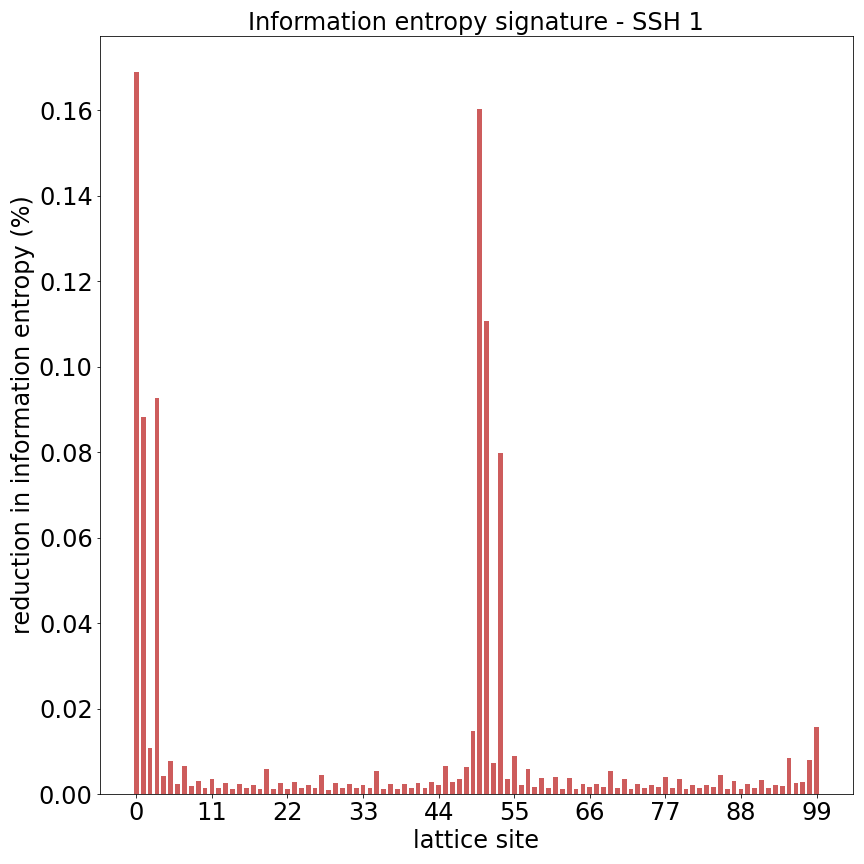
\includegraphics[width=0.49\textwidth]{./ssh1/periodic_100_6561/plot_feature_importances.png}}\quad
\subfigure[]{\label{feature_importances_ssh2}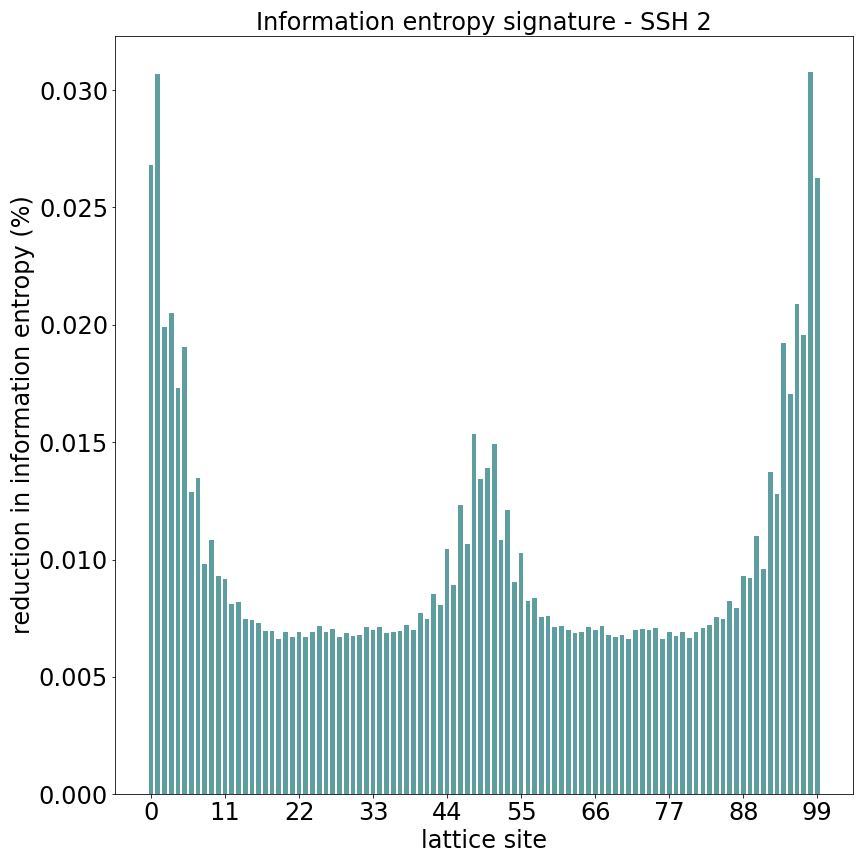
\includegraphics[width=0.49\textwidth]{./ssh2/periodic_100_6561/plot_feature_importances.png}}\quad
\caption{Information entropy signatures of the topological phase transitions from experiments 1 and 2. (a) In experiment 1, the two sharp peaks in the Shannon entropy signal account for approximately 70\% of reduction in information entropy. These two peaks correspond to the lattice sites $S_1$. (b) In experiment 2, the three visible peaks account for approximately 30\% of reduction in information entropy. These three peaks are located along lattice sites $S_2$.}
\label{feature_importances}
\end{figure}

\begin{thebibliography}{10}
\urlstyle{rm}
\expandafter\ifx\csname url\endcsname\relax
  \def\url#1{\texttt{#1}}\fi
\expandafter\ifx\csname urlprefix\endcsname\relax\def\urlprefix{URL }\fi
\expandafter\ifx\csname doiprefix\endcsname\relax\def\doiprefix{DOI: }\fi
\providecommand{\bibinfo}[2]{#2}
\providecommand{\eprint}[2][]{\url{#2}}

\bibitem{RevModPhys.82.3045}
\bibinfo{author}{Hasan, M.~Z.} \& \bibinfo{author}{Kane, C.~L.}
\newblock \bibinfo{journal}{\bibinfo{title}{Colloquium: Topological
  insulators}}.
\newblock {\emph{\JournalTitle{Rev. Mod. Phys.}}}
  \textbf{\bibinfo{volume}{82}}, \bibinfo{pages}{3045--3067}
  (\bibinfo{year}{2010}).

\bibitem{CONTINENTINO2017A1}
\bibinfo{author}{Continentino, M.~A.}
\newblock \bibinfo{journal}{\bibinfo{title}{Topological phase transitions}}.
\newblock {\emph{\JournalTitle{Physica B: Condensed Matter}}}
  \textbf{\bibinfo{volume}{505}}, \bibinfo{pages}{A1 -- A2}
  (\bibinfo{year}{2017}).

\bibitem{PhysRevB.95.094509}
\bibinfo{author}{Puel, T.~O.}, \bibinfo{author}{Sacramento, P.~D.} \&
  \bibinfo{author}{Continentino, M.~A.}
\newblock \bibinfo{journal}{\bibinfo{title}{$4\ensuremath{\pi}$ josephson
  currents in junctions of hybridized multiband superconductors}}.
\newblock {\emph{\JournalTitle{Phys. Rev. B}}} \textbf{\bibinfo{volume}{95}},
  \bibinfo{pages}{094509} (\bibinfo{year}{2017}).

\bibitem{PhysRevE.97.012107}
\bibinfo{author}{Griffith, M.~A.} \& \bibinfo{author}{Continentino, M.~A.}
\newblock \bibinfo{journal}{\bibinfo{title}{Casimir amplitudes in topological
  quantum phase transitions}}.
\newblock {\emph{\JournalTitle{Phys. Rev. E}}} \textbf{\bibinfo{volume}{97}},
  \bibinfo{pages}{012107} (\bibinfo{year}{2018}).

\bibitem{ryu2010topological}
\bibinfo{author}{Ryu, S.}, \bibinfo{author}{Schnyder, A.~P.},
  \bibinfo{author}{Furusaki, A.} \& \bibinfo{author}{Ludwig, A.~W.}
\newblock \bibinfo{journal}{\bibinfo{title}{Topological insulators and
  superconductors: tenfold way and dimensional hierarchy}}.
\newblock {\emph{\JournalTitle{New Journal of Physics}}}
  \textbf{\bibinfo{volume}{12}}, \bibinfo{pages}{065010}
  (\bibinfo{year}{2010}).

\bibitem{atala2013direct}
\bibinfo{author}{Atala, M.} \emph{et~al.}
\newblock \bibinfo{journal}{\bibinfo{title}{Direct measurement of the zak phase
  in topological bloch bands}}.
\newblock {\emph{\JournalTitle{Nature Physics}}} \textbf{\bibinfo{volume}{9}},
  \bibinfo{pages}{795} (\bibinfo{year}{2013}).

\bibitem{Stuhl1514}
\bibinfo{author}{Stuhl, B.~K.}, \bibinfo{author}{Lu, H.-I.},
  \bibinfo{author}{Aycock, L.~M.}, \bibinfo{author}{Genkina, D.} \&
  \bibinfo{author}{Spielman, I.~B.}
\newblock \bibinfo{journal}{\bibinfo{title}{Visualizing edge states with an
  atomic bose gas in the quantum hall regime}}.
\newblock {\emph{\JournalTitle{Science}}} \textbf{\bibinfo{volume}{349}},
  \bibinfo{pages}{1514--1518} (\bibinfo{year}{2015}).

\bibitem{leder2016real}
\bibinfo{author}{Leder, M.} \emph{et~al.}
\newblock \bibinfo{journal}{\bibinfo{title}{Real-space imaging of a
  topologically protected edge state with ultracold atoms in an
  amplitude-chirped optical lattice}}.
\newblock {\emph{\JournalTitle{Nature communications}}}
  \textbf{\bibinfo{volume}{7}}, \bibinfo{pages}{13112} (\bibinfo{year}{2016}).

\bibitem{goldman2016topological}
\bibinfo{author}{Goldman, N.}, \bibinfo{author}{Budich, J.} \&
  \bibinfo{author}{Zoller, P.}
\newblock \bibinfo{journal}{\bibinfo{title}{Topological quantum matter with
  ultracold gases in optical lattices}}.
\newblock {\emph{\JournalTitle{Nature Physics}}} \textbf{\bibinfo{volume}{12}},
  \bibinfo{pages}{639} (\bibinfo{year}{2016}).

\bibitem{meier2016observation}
\bibinfo{author}{Meier, E.~J.}, \bibinfo{author}{An, F.~A.} \&
  \bibinfo{author}{Gadway, B.}
\newblock \bibinfo{journal}{\bibinfo{title}{Observation of the topological
  soliton state in the su--schrieffer--heeger model}}.
\newblock {\emph{\JournalTitle{Nature communications}}}
  \textbf{\bibinfo{volume}{7}}, \bibinfo{pages}{13986} (\bibinfo{year}{2016}).

\bibitem{hafezi2013imaging}
\bibinfo{author}{Hafezi, M.}, \bibinfo{author}{Mittal, S.},
  \bibinfo{author}{Fan, J.}, \bibinfo{author}{Migdall, A.} \&
  \bibinfo{author}{Taylor, J.}
\newblock \bibinfo{journal}{\bibinfo{title}{Imaging topological edge states in
  silicon photonics}}.
\newblock {\emph{\JournalTitle{Nature Photonics}}}
  \textbf{\bibinfo{volume}{7}}, \bibinfo{pages}{1001} (\bibinfo{year}{2013}).

\bibitem{lu2016topological}
\bibinfo{author}{Lu, L.}, \bibinfo{author}{Joannopoulos, J.~D.} \&
  \bibinfo{author}{Solja{\v{c}}i{\'c}, M.}
\newblock \bibinfo{journal}{\bibinfo{title}{Topological states in photonic
  systems}}.
\newblock {\emph{\JournalTitle{Nature Physics}}} \textbf{\bibinfo{volume}{12}},
  \bibinfo{pages}{626} (\bibinfo{year}{2016}).

\bibitem{PhysRevX.5.031011}
\bibinfo{author}{Peano, V.}, \bibinfo{author}{Brendel, C.},
  \bibinfo{author}{Schmidt, M.} \& \bibinfo{author}{Marquardt, F.}
\newblock \bibinfo{journal}{\bibinfo{title}{Topological phases of sound and
  light}}.
\newblock {\emph{\JournalTitle{Phys. Rev. X}}} \textbf{\bibinfo{volume}{5}},
  \bibinfo{pages}{031011} (\bibinfo{year}{2015}).

\bibitem{kitagawa2012observation}
\bibinfo{author}{Kitagawa, T.} \emph{et~al.}
\newblock \bibinfo{journal}{\bibinfo{title}{Observation of topologically
  protected bound states in photonic quantum walks}}.
\newblock {\emph{\JournalTitle{Nature communications}}}
  \textbf{\bibinfo{volume}{3}}, \bibinfo{pages}{882} (\bibinfo{year}{2012}).

\bibitem{cardano2016statistical}
\bibinfo{author}{Cardano, F.} \emph{et~al.}
\newblock \bibinfo{journal}{\bibinfo{title}{Statistical moments of quantum-walk
  dynamics reveal topological quantum transitions}}.
\newblock {\emph{\JournalTitle{Nature communications}}}
  \textbf{\bibinfo{volume}{7}}, \bibinfo{pages}{11439} (\bibinfo{year}{2016}).

\bibitem{PhysRevX.7.031023}
\bibinfo{author}{Flurin, E.} \emph{et~al.}
\newblock \bibinfo{journal}{\bibinfo{title}{Observing topological invariants
  using quantum walks in superconducting circuits}}.
\newblock {\emph{\JournalTitle{Phys. Rev. X}}} \textbf{\bibinfo{volume}{7}},
  \bibinfo{pages}{031023} (\bibinfo{year}{2017}).

\bibitem{soluyanov2015type}
\bibinfo{author}{Soluyanov, A.~A.} \emph{et~al.}
\newblock \bibinfo{journal}{\bibinfo{title}{Type-ii weyl semimetals}}.
\newblock {\emph{\JournalTitle{Nature}}} \textbf{\bibinfo{volume}{527}},
  \bibinfo{pages}{495} (\bibinfo{year}{2015}).

\bibitem{PhysRevX.5.031013}
\bibinfo{author}{Lv, B.~Q.} \emph{et~al.}
\newblock \bibinfo{journal}{\bibinfo{title}{Experimental discovery of weyl
  semimetal taas}}.
\newblock {\emph{\JournalTitle{Phys. Rev. X}}} \textbf{\bibinfo{volume}{5}},
  \bibinfo{pages}{031013} (\bibinfo{year}{2015}).

\bibitem{PhysRevLett.42.1698}
\bibinfo{author}{Su, W.~P.}, \bibinfo{author}{Schrieffer, J.~R.} \&
  \bibinfo{author}{Heeger, A.~J.}
\newblock \bibinfo{journal}{\bibinfo{title}{Solitons in polyacetylene}}.
\newblock {\emph{\JournalTitle{Phys. Rev. Lett.}}}
  \textbf{\bibinfo{volume}{42}}, \bibinfo{pages}{1698--1701}
  (\bibinfo{year}{1979}).

\bibitem{maffei2018topological}
\bibinfo{author}{Maffei, M.}, \bibinfo{author}{Dauphin, A.},
  \bibinfo{author}{Cardano, F.}, \bibinfo{author}{Lewenstein, M.} \&
  \bibinfo{author}{Massignan, P.}
\newblock \bibinfo{journal}{\bibinfo{title}{Topological characterization of
  chiral models through their long time dynamics}}.
\newblock {\emph{\JournalTitle{New Journal of Physics}}}
  \textbf{\bibinfo{volume}{20}}, \bibinfo{pages}{013023}
  (\bibinfo{year}{2018}).

\bibitem{RevModPhys.73.681}
\bibinfo{author}{Heeger, A.~J.}
\newblock \bibinfo{journal}{\bibinfo{title}{Nobel lecture: Semiconducting and
  metallic polymers: The fourth generation of polymeric materials}}.
\newblock {\emph{\JournalTitle{Rev. Mod. Phys.}}}
  \textbf{\bibinfo{volume}{73}}, \bibinfo{pages}{681--700}
  (\bibinfo{year}{2001}).

\bibitem{kane2014topological}
\bibinfo{author}{Kane, C.} \& \bibinfo{author}{Lubensky, T.}
\newblock \bibinfo{journal}{\bibinfo{title}{Topological boundary modes in
  isostatic lattices}}.
\newblock {\emph{\JournalTitle{Nature Physics}}} \textbf{\bibinfo{volume}{10}},
  \bibinfo{pages}{39} (\bibinfo{year}{2014}).

\bibitem{Chen13004}
\bibinfo{author}{Chen, B. G.-g.}, \bibinfo{author}{Upadhyaya, N.} \&
  \bibinfo{author}{Vitelli, V.}
\newblock \bibinfo{journal}{\bibinfo{title}{Nonlinear conduction via solitons
  in a topological mechanical insulator}}.
\newblock {\emph{\JournalTitle{Proceedings of the National Academy of
  Sciences}}} \textbf{\bibinfo{volume}{111}}, \bibinfo{pages}{13004--13009}
  (\bibinfo{year}{2014}).

\bibitem{carrasquilla2017machine}
\bibinfo{author}{Carrasquilla, J.} \& \bibinfo{author}{Melko, R.~G.}
\newblock \bibinfo{journal}{\bibinfo{title}{Machine learning phases of
  matter}}.
\newblock {\emph{\JournalTitle{Nature Physics}}} \textbf{\bibinfo{volume}{13}},
  \bibinfo{pages}{431} (\bibinfo{year}{2017}).

\bibitem{PhysRevX.7.031038}
\bibinfo{author}{Ch'ng, K.}, \bibinfo{author}{Carrasquilla, J.},
  \bibinfo{author}{Melko, R.~G.} \& \bibinfo{author}{Khatami, E.}
\newblock \bibinfo{journal}{\bibinfo{title}{Machine learning phases of strongly
  correlated fermions}}.
\newblock {\emph{\JournalTitle{Phys. Rev. X}}} \textbf{\bibinfo{volume}{7}},
  \bibinfo{pages}{031038} (\bibinfo{year}{2017}).

\bibitem{PhysRevB.94.195105}
\bibinfo{author}{Wang, L.}
\newblock \bibinfo{journal}{\bibinfo{title}{Discovering phase transitions with
  unsupervised learning}}.
\newblock {\emph{\JournalTitle{Phys. Rev. B}}} \textbf{\bibinfo{volume}{94}},
  \bibinfo{pages}{195105} (\bibinfo{year}{2016}).

\bibitem{broecker2017machine}
\bibinfo{author}{Broecker, P.}, \bibinfo{author}{Carrasquilla, J.},
  \bibinfo{author}{Melko, R.~G.} \& \bibinfo{author}{Trebst, S.}
\newblock \bibinfo{journal}{\bibinfo{title}{Machine learning quantum phases of
  matter beyond the fermion sign problem}}.
\newblock {\emph{\JournalTitle{Scientific reports}}}
  \textbf{\bibinfo{volume}{7}}, \bibinfo{pages}{8823} (\bibinfo{year}{2017}).

\bibitem{van2017learning}
\bibinfo{author}{Van~Nieuwenburg, E.~P.}, \bibinfo{author}{Liu, Y.-H.} \&
  \bibinfo{author}{Huber, S.~D.}
\newblock \bibinfo{journal}{\bibinfo{title}{Learning phase transitions by
  confusion}}.
\newblock {\emph{\JournalTitle{Nature Physics}}} \textbf{\bibinfo{volume}{13}},
  \bibinfo{pages}{435} (\bibinfo{year}{2017}).

\bibitem{PhysRevLett.120.066401}
\bibinfo{author}{Zhang, P.}, \bibinfo{author}{Shen, H.} \&
  \bibinfo{author}{Zhai, H.}
\newblock \bibinfo{journal}{\bibinfo{title}{Machine learning topological
  invariants with neural networks}}.
\newblock {\emph{\JournalTitle{Phys. Rev. Lett.}}}
  \textbf{\bibinfo{volume}{120}}, \bibinfo{pages}{066401}
  (\bibinfo{year}{2018}).

\bibitem{PhysRevB.98.085402}
\bibinfo{author}{Sun, N.}, \bibinfo{author}{Yi, J.}, \bibinfo{author}{Zhang,
  P.}, \bibinfo{author}{Shen, H.} \& \bibinfo{author}{Zhai, H.}
\newblock \bibinfo{journal}{\bibinfo{title}{Deep learning topological
  invariants of band insulators}}.
\newblock {\emph{\JournalTitle{Phys. Rev. B}}} \textbf{\bibinfo{volume}{98}},
  \bibinfo{pages}{085402} (\bibinfo{year}{2018}).

\bibitem{PhysRevB.97.174435}
\bibinfo{author}{Suchsland, P.} \& \bibinfo{author}{Wessel, S.}
\newblock \bibinfo{journal}{\bibinfo{title}{Parameter diagnostics of phases and
  phase transition learning by neural networks}}.
\newblock {\emph{\JournalTitle{Phys. Rev. B}}} \textbf{\bibinfo{volume}{97}},
  \bibinfo{pages}{174435} (\bibinfo{year}{2018}).

\bibitem{PhysRevLett.118.216401}
\bibinfo{author}{Zhang, Y.} \& \bibinfo{author}{Kim, E.-A.}
\newblock \bibinfo{journal}{\bibinfo{title}{Quantum loop topography for machine
  learning}}.
\newblock {\emph{\JournalTitle{Phys. Rev. Lett.}}}
  \textbf{\bibinfo{volume}{118}}, \bibinfo{pages}{216401}
  (\bibinfo{year}{2017}).

\bibitem{PhysRevLett.120.257204}
\bibinfo{author}{Venderley, J.}, \bibinfo{author}{Khemani, V.} \&
  \bibinfo{author}{Kim, E.-A.}
\newblock \bibinfo{journal}{\bibinfo{title}{Machine learning out-of-equilibrium
  phases of matter}}.
\newblock {\emph{\JournalTitle{Phys. Rev. Lett.}}}
  \textbf{\bibinfo{volume}{120}}, \bibinfo{pages}{257204}
  (\bibinfo{year}{2018}).

\bibitem{ohtsuki2017deep}
\bibinfo{author}{Ohtsuki, T.} \& \bibinfo{author}{Ohtsuki, T.}
\newblock \bibinfo{journal}{\bibinfo{title}{Deep learning the quantum phase
  transitions in random electron systems: Applications to three dimensions}}.
\newblock {\emph{\JournalTitle{Journal of the Physical Society of Japan}}}
  \textbf{\bibinfo{volume}{86}}, \bibinfo{pages}{044708}
  (\bibinfo{year}{2017}).

\bibitem{PhysRevB.97.205110}
\bibinfo{author}{Yoshioka, N.}, \bibinfo{author}{Akagi, Y.} \&
  \bibinfo{author}{Katsura, H.}
\newblock \bibinfo{journal}{\bibinfo{title}{Learning disordered topological
  phases by statistical recovery of symmetry}}.
\newblock {\emph{\JournalTitle{Phys. Rev. B}}} \textbf{\bibinfo{volume}{97}},
  \bibinfo{pages}{205110} (\bibinfo{year}{2018}).

\bibitem{PhysRevB.96.195145}
\bibinfo{author}{Deng, D.-L.}, \bibinfo{author}{Li, X.} \&
  \bibinfo{author}{Das~Sarma, S.}
\newblock \bibinfo{journal}{\bibinfo{title}{Machine learning topological
  states}}.
\newblock {\emph{\JournalTitle{Phys. Rev. B}}} \textbf{\bibinfo{volume}{96}},
  \bibinfo{pages}{195145} (\bibinfo{year}{2017}).

\bibitem{PhysRevB.97.134109}
\bibinfo{author}{Huembeli, P.}, \bibinfo{author}{Dauphin, A.} \&
  \bibinfo{author}{Wittek, P.}
\newblock \bibinfo{journal}{\bibinfo{title}{Identifying quantum phase
  transitions with adversarial neural networks}}.
\newblock {\emph{\JournalTitle{Phys. Rev. B}}} \textbf{\bibinfo{volume}{97}},
  \bibinfo{pages}{134109} (\bibinfo{year}{2018}).

\bibitem{PhysRevB.97.115453}
\bibinfo{author}{Carvalho, D.}, \bibinfo{author}{Garc\'{\i}a-Mart\'{\i}nez,
  N.~A.}, \bibinfo{author}{Lado, J.~L.} \&
  \bibinfo{author}{Fern\'andez-Rossier, J.}
\newblock \bibinfo{journal}{\bibinfo{title}{Real-space mapping of topological
  invariants using artificial neural networks}}.
\newblock {\emph{\JournalTitle{Phys. Rev. B}}} \textbf{\bibinfo{volume}{97}},
  \bibinfo{pages}{115453} (\bibinfo{year}{2018}).

\bibitem{PhysRevB.96.245119}
\bibinfo{author}{Zhang, Y.}, \bibinfo{author}{Melko, R.~G.} \&
  \bibinfo{author}{Kim, E.-A.}
\newblock \bibinfo{journal}{\bibinfo{title}{Machine learning ${\mathbb{z}}_{2}$
  quantum spin liquids with quasiparticle statistics}}.
\newblock {\emph{\JournalTitle{Phys. Rev. B}}} \textbf{\bibinfo{volume}{96}},
  \bibinfo{pages}{245119} (\bibinfo{year}{2017}).

\bibitem{rodriguez2018identifying}
\bibinfo{author}{Rodriguez-Nieva, J.~F.} \& \bibinfo{author}{Scheurer, M.~S.}
\newblock \bibinfo{journal}{\bibinfo{title}{Identifying topological order via
  unsupervised machine learning}}.
\newblock {\emph{\JournalTitle{arXiv preprint arXiv:1805.05961}}}
  (\bibinfo{year}{2018}).

\bibitem{breiman2017classification}
\bibinfo{author}{Breiman, L.}, \bibinfo{author}{Friedman, J.},
  \bibinfo{author}{Stone, C.~J.} \& \bibinfo{author}{Olshen, R.~A.}
\newblock \emph{\bibinfo{title}{Classification and regression trees}}
  (\bibinfo{publisher}{Chapman and Hall/CRC, London, UK},
  \bibinfo{year}{1984}).

\bibitem{Breiman2001}
\bibinfo{author}{Breiman, L.}
\newblock \bibinfo{journal}{\bibinfo{title}{Random forests}}.
\newblock {\emph{\JournalTitle{Machine Learning}}}
  \textbf{\bibinfo{volume}{45}}, \bibinfo{pages}{5--32} (\bibinfo{year}{2001}).

\bibitem{friedman2001elements}
\bibinfo{author}{Friedman, J.}, \bibinfo{author}{Hastie, T.} \&
  \bibinfo{author}{Tibshirani, R.}
\newblock \emph{\bibinfo{title}{The elements of statistical learning}}
  (\bibinfo{publisher}{Springer New York, NY, USA}, \bibinfo{year}{2001}).

\bibitem{PhysRevB.84.241106}
\bibinfo{author}{Bianco, R.} \& \bibinfo{author}{Resta, R.}
\newblock \bibinfo{journal}{\bibinfo{title}{Mapping topological order in
  coordinate space}}.
\newblock {\emph{\JournalTitle{Phys. Rev. B}}} \textbf{\bibinfo{volume}{84}},
  \bibinfo{pages}{241106} (\bibinfo{year}{2011}).

\bibitem{caio2019topological}
\bibinfo{author}{Caio, M.~D.}, \bibinfo{author}{M{\"o}ller, G.},
  \bibinfo{author}{Cooper, N.~R.} \& \bibinfo{author}{Bhaseen, M.}
\newblock \bibinfo{journal}{\bibinfo{title}{Topological marker currents in
  chern insulators}}.
\newblock {\emph{\JournalTitle{Nature Physics}}} \bibinfo{pages}{1}
  (\bibinfo{year}{2019}).

\bibitem{carlsson2009topology}
\bibinfo{author}{Carlsson, G.}
\newblock \bibinfo{journal}{\bibinfo{title}{Topology and data}}.
\newblock {\emph{\JournalTitle{Bulletin of the American Mathematical Society}}}
  \textbf{\bibinfo{volume}{46}}, \bibinfo{pages}{255--308}
  (\bibinfo{year}{2009}).

\bibitem{wasserman2018topological}
\bibinfo{author}{Wasserman, L.}
\newblock \bibinfo{journal}{\bibinfo{title}{Topological data analysis}}.
\newblock {\emph{\JournalTitle{Annual Review of Statistics and Its
  Application}}} \textbf{\bibinfo{volume}{5}}, \bibinfo{pages}{501--532}
  (\bibinfo{year}{2018}).

\bibitem{wang2005adaptive}
\bibinfo{author}{Wang, J.}, \bibinfo{author}{Zhang, Z.} \&
  \bibinfo{author}{Zha, H.}
\newblock \bibinfo{title}{Adaptive manifold learning}.
\newblock In \emph{\bibinfo{booktitle}{Advances in neural information
  processing systems}}, \bibinfo{pages}{1473--1480} (\bibinfo{year}{2005}).

\bibitem{lin2008riemannian}
\bibinfo{author}{Lin, T.} \& \bibinfo{author}{Zha, H.}
\newblock \bibinfo{journal}{\bibinfo{title}{Riemannian manifold learning}}.
\newblock {\emph{\JournalTitle{IEEE Transactions on Pattern Analysis and
  Machine Intelligence}}} \textbf{\bibinfo{volume}{30}},
  \bibinfo{pages}{796--809} (\bibinfo{year}{2008}).

\bibitem{belkin2003problems}
\bibinfo{author}{Belkin, M.}
\newblock \emph{\bibinfo{title}{Problems of learning on manifolds}}
  (\bibinfo{publisher}{The University of Chicago, Chicago, IL, USA},
  \bibinfo{year}{2003}).

\bibitem{asboth2016short}
\bibinfo{author}{Asb{\'o}th, J.~K.}, \bibinfo{author}{Oroszl{\'a}ny, L.} \&
  \bibinfo{author}{P{\'a}lyi, A.}
\newblock \bibinfo{journal}{\bibinfo{title}{A short course on topological
  insulators}}.
\newblock {\emph{\JournalTitle{Lecture notes in physics}}}
  \textbf{\bibinfo{volume}{919}} (\bibinfo{year}{2016}).

\bibitem{goodfellow2016deep}
\bibinfo{author}{Goodfellow, I.}, \bibinfo{author}{Bengio, Y.} \&
  \bibinfo{author}{Courville, A.}
\newblock \emph{\bibinfo{title}{Deep learning}} (\bibinfo{publisher}{MIT press,
  Cambridge, MA, USA}, \bibinfo{year}{2016}).

\bibitem{bishop2006pattern}
\bibinfo{author}{Bishop, C.~M.}
\newblock \emph{\bibinfo{title}{Pattern recognition and machine learning}}
  (\bibinfo{publisher}{Springer New York, NY, USA}, \bibinfo{year}{2006}).

\bibitem{cayton2005algorithms}
\bibinfo{author}{Cayton, L.}
\newblock \bibinfo{journal}{\bibinfo{title}{Algorithms for manifold learning}}.
\newblock {\emph{\JournalTitle{Univ. of California at San Diego Tech. Rep}}}
  \textbf{\bibinfo{volume}{12}}, \bibinfo{pages}{1} (\bibinfo{year}{2005}).

\bibitem{narayanan2010sample}
\bibinfo{author}{Narayanan, H.} \& \bibinfo{author}{Mitter, S.}
\newblock \bibinfo{title}{Sample complexity of testing the manifold
  hypothesis}.
\newblock In \emph{\bibinfo{booktitle}{Advances in Neural Information
  Processing Systems}}, \bibinfo{pages}{1786--1794} (\bibinfo{year}{2010}).

\bibitem{rifai2011manifold}
\bibinfo{author}{Rifai, S.}, \bibinfo{author}{Dauphin, Y.~N.},
  \bibinfo{author}{Vincent, P.}, \bibinfo{author}{Bengio, Y.} \&
  \bibinfo{author}{Muller, X.}
\newblock \bibinfo{title}{The manifold tangent classifier}.
\newblock In \emph{\bibinfo{booktitle}{Advances in Neural Information
  Processing Systems}}, \bibinfo{pages}{2294--2302} (\bibinfo{year}{2011}).

\end{thebibliography}
%\bibliographystyle{plain}
%\bibliographystyle{ieeetr}

\section*{Acknowledgements}

We thank S. E. Rowley, J. F. de Oliveira, T. Micklitz and M. A. Continentino for insightful discussions and S. E. Rowley for carefully reading the manuscript and suggesting improvements. N. L. Holanda acknowledges financial support from CENPES/Petrobr\'as/CBPF. M. A. R. Griffith acknowledges financial support from Capes. N. L. Holanda is grateful to the Theory of Condensed Matter and Quantum Materials groups at the Cavendish Laboratory and the Quantum Information Group at CBPF.


\section*{Author contributions}

Both authors of this work contributed equally to its realization at all stages.

\section*{Competing financial interests}

The authors declare no competing financial or non-financial interests.

\section*{Additional information}

Correspondence and requests for materials should be addressed to N. L. Holanda. The source code used to run simulations is available on \href{https://github.com/linneuholanda/ml_topological_phases_in_real_space}{Github}.




\newpage

\begin{figure}
  \centering
  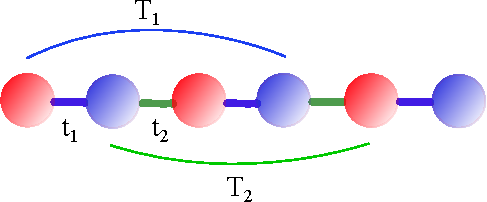
\includegraphics[width=.37\textwidth]{./phase_diagrams/ssh_model.pdf}
  \caption{Schematic set-up of a 1D SSH system. Here $t_1$ and $t_2$ are nearest-neighbor hoppings while $T_1$ and $T_2$ are second nearest-neighbor hoppings.}
\label{fig:model}
\end{figure}

\begin{figure}%[h!]
  \centering
  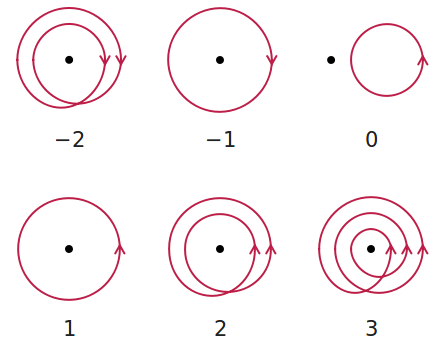
\includegraphics[width=.37\textwidth]{./phase_diagrams/winding.png}
  \caption{Winding number. The winding number of a closed, oriented curve with respect to a reference point is a topological invariant that counts how many times the curve winds around the point. Picture credits: Jim Belk, public domain.}
\label{fig:winding}
\end{figure}


\section*{Supplementary Material}
\subsection*{The SSH model}
\label{sshapp}

The SSH model \cite{asboth2016short} describes the movement of free electrons along a dimerized chain whose basic units consist of two distinct atoms. This movement, usually called ``hopping'' in the literature, can be made either between atoms in a unit cell or between unit cells, and the allowed hopping rules for a given system completely determine its Hamiltonian. This is because the kinetic energies of the electrons are parameterized by a vector of real numbers $\mathbf{t}$ that also encodes hopping terms, thus allowing for a compact mathematical description of a Hamiltonian in terms of creation/annihilation operators as
\begin{equation}
\label{SSH}
\hat{H}(\mathbf{t})=\mathbf{c}^{\dagger}H(\mathbf{t})\mathbf{c}
\end{equation}
where the column vector
\begin{equation*}
\mathbf{c} =\Big(c^{A}_1,c^{B}_1,\cdots,c^{A}_\frac{N}{2},c^{B}_\frac{N}{2}\Big)^T
\end{equation*}
contains annihilation operators $c^{A(B)}_p$ that erase electrons at atom A (B) and lattice site $p$ and similarly the row vector
\begin{equation*}
\mathbf{c}^\dagger =\Big(c^{A\dagger}_1,c^{B\dagger}_1,\cdots,c^{A\dagger}_\frac{N}{2},c^{B\dagger}_\frac{N}{2}\Big)
\end{equation*}
contains creation operators $c^{A(B)\dagger}_p$ that produce electrons at atom A (B) and lattice site $p$. Please note that $N$ is twice the number of unit cells in the chain and therefore an even integer.

The convenience of equation \eqref{SSH} is that all information about a system such as its eigenstates and eigenenergies can be recovered from the $N\times N$ matrix $H(\mathbf{t})$. We can thus think of the vectors $\mathbf{t}$ in parameter space as very compact representations of SSH models: each point in $\mathbf{t}$-space can be mapped to a $N\times N$ matrix $H(\mathbf{t})$ whose eigenvectors and eigenvalues can then be computed, as is usually done in quantum mechanics. As an example, a general matrix $H(\mathbf{t})$ describing a SSH system with hoppings between nearest and second nearest neighbors is given by
\begin{equation}\label{hmatrix}
H(t_1,t_2,T_1,T_2)=\left(
  \begin{array}{cccccc}
    0 & t_1 & 0 & T_1 & 0 & \cdots \\
    t_1 & 0 & t_2& 0 & T_2 & \cdots\\
    0 & t_2 & 0 & t_1 & 0 & \cdots\\
    T_1 & 0 & t_1 & 0 & t_2 & \cdots\\
    0 & T_2 & 0 & t_2 &  0& \cdots\\
    \vdots & \vdots    & \vdots & \vdots &  \vdots & \ddots\\
  \end{array}
  \right)_{N \times N}.
\end{equation}
Knowing the vector $\mathbf{t}=(t_1,t_2,T_1,T_2)$ corresponding to a particular system described by the Hamiltonian in equation \eqref{hmatrix} should suffice to compute any of its physical properties, including its topological phase. Figure \ref{fig:model} depicts a SSH system described by equation \eqref{hmatrix}.

The reason why topological materials garnered so much interest in recent years is that their physical properties are topologically robust.
This means that these properties are stable under continuous (i.e., adiabatic) mathematical operations performed on the system's underlying wave functions. This topological robustness is expressed theoretically in terms of a topological invariant that characterizes different phases of a system. In the particular case of the SSH model, the topological invariant used to classify the topological phases is the winding number.

The winding number is a topological property of any closed, oriented curve that measures how many times the curve winds around a point that does not belong to itself. It can be any integer and is usually chosen to be positive when the curve winds in counterclockwise motion with respect to the reference point (equivalently, when a closed, oriented curve winds in clockwise motion around a reference point its winding number is negative). Figure \ref{fig:winding} shows several closed, oriented curves and their winding numbers computed with respect to a given point.

An interesting property of topological invariants like the winding number is that they are a global feature of geometric objects: for each of the curves in figure \ref{fig:winding} for example the winding number is a property of the whole curve that cannot be defined locally for each of its points. This fundamental characteristic of topological invariants makes the study of topological phases of matter from local lattice data a very challenging task.   

For SSH systems with translational symmetry like the finite systems with periodic boundary conditions investigated in the article, the winding number is usually computed in wavevector space via
\begin{equation}\label{winding_number}
W=\frac{1}{4\pi i}\int_0^{2\pi} dk Tr( \sigma_3 H(k)^{-1} \partial_k H(k)),
\end{equation}
where $H(k)$ is the kernel in wavevector space of a Hamiltonian $\hat{H}$$($$\mathbf{t}$$)$ and $\sigma_3$ is the chiral operator. Equation \eqref{winding_number} can be evaluated for several Hamiltonians by varying the parameter $\mathbf{t}$, resulting in phase diagrams in parameter space like the ones shown in figure \ref{fig:phasediagrams}.

\begin{figure}
\centering
\subfigure[]{\label{less_feat:a}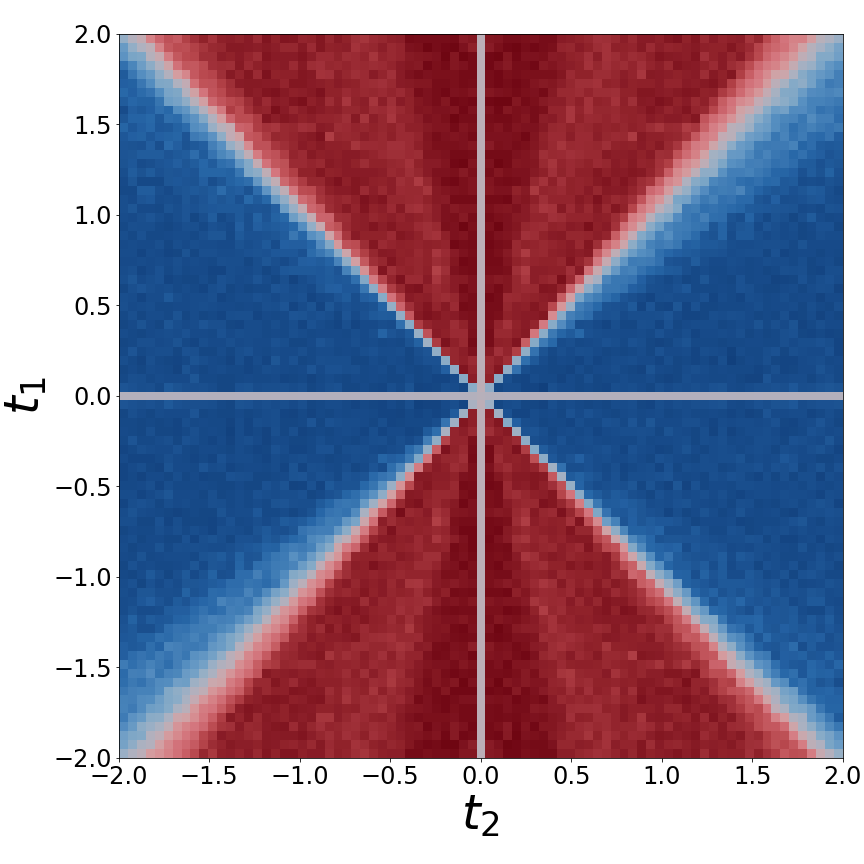
\includegraphics[width=.49\textwidth]{./ssh1/periodic_less_100_6561/merge_imshow_winding_grids_second_sim.png}}
\subfigure[]{\label{less_feat:b}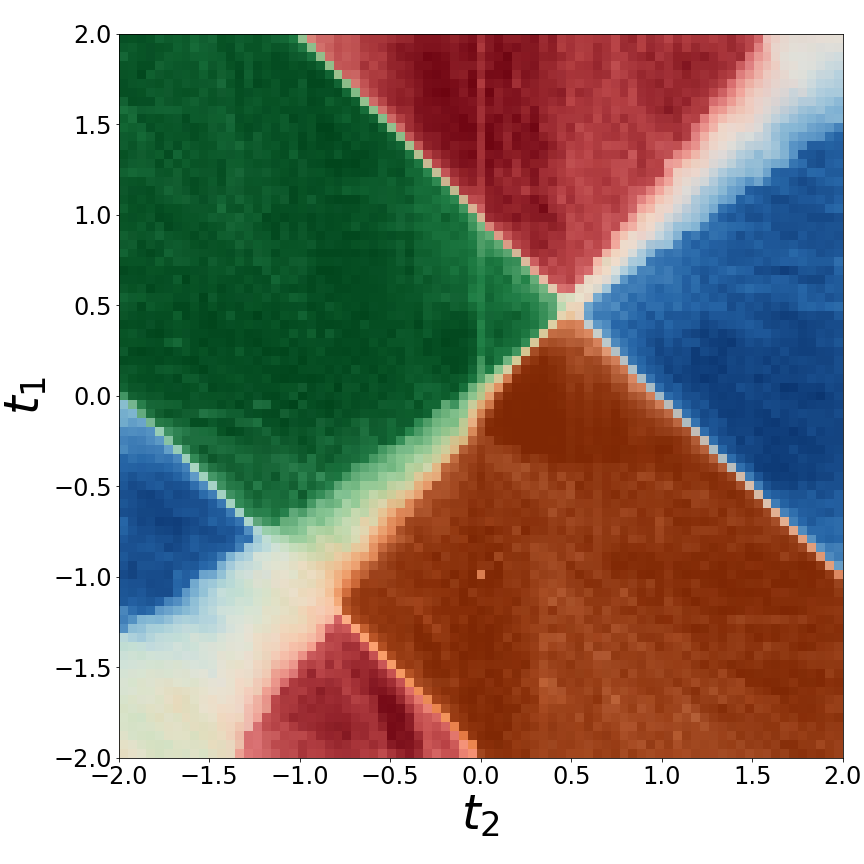
\includegraphics[width=.49\textwidth]{./ssh2/periodic_less_100_6561/merge_imshow_winding_grids_sim.png}}
\caption{Phase diagrams learned from most relevant lattice sites. (a) Phase diagram learned by a combination of decision trees with eigenvector ensembling in experiment 1 using only lattice sites $S'_1$ = (0, 50, 51, 99). The accuracy achieved for Hamiltonians in the test set using only the four lattice sites in $S'_1$ was approximately 95\%.  (b) Phase diagram learned by a combination of random forests with eigenvector ensembling in experiment 2 using only lattice sites $S'_2$ = (0, 1, 3, 48, 50, 51, 96, 98, 99). The accuracy achieved for Hamiltonians in the test set using only the nine lattice sites in $S'_2$ was approximately 74\%.}
\label{less_feat}
\end{figure}

\subsection*{Learning topological phases from real space data}

The main motivations for developing a data-driven approach based on real space are that wavevector space computations such as eq. \eqref{winding_number} are only possible for systems with translational symmetry, which many physical systems of current interest (e.g. disordered systems in condensed matter) do not have. Moreover, since real space and wavevector space eigenvectors are related by Fourier transforms, the latter are essentially delocalized and therefore so is any information recovered from them. We argue here that a data-driven approach based on real space offers a viable alternative to wavevector space computations that addresses these shortcomings.

Our reasoning goes as follows. First, while the topological invariants that characterize distinct topological phases are usually computed in wavevector space, the topological properties of a Hamiltonian are the same regardless of the basis in Hilbert space used to represent it. Thus, information on the topological phase of a Hamiltonian should still be available when it is represented in real lattice space. Second, even though the topological properties of a Hamiltonian are global, meaning that in general they cannot be said to be localized at a particular lattice site, in parameter space topology is indeed a local property: knowing the vector $\mathbf{t}$ associated with a Hamiltonian completely determines its topological phase.

In a data-driven approach, locality is often exploited by means of a local constancy hypothesis \cite{goodfellow2016deep}. Mathematically, this policy prescribes the value of a function $W(\mathbf{t}')$ at points where it is unknown in a vicinity of a data point $\mathbf{t}$ as approximately equal to its known value $W(\mathbf{t})$,
\begin{equation}
\label{localconstancy}
W(\mathbf{t} + \boldsymbol{\delta}) \approx W(\mathbf{t}).
\end{equation}

That such a policy will be successful in classifying topological phases in parameter space can be visualized in figure \ref{fig:phasediagrams}, where we draw phase diagrams of SSH models with first-neighbor (figure \ref{ssh1}) and first- and second-neighbor (figure \ref{ssh2}) hoppings. In figure \ref{ssh1} for example, it is clear that knowing a particular Hamiltonian $H(t_1,t_2)$ with winding number $W = 0$ (that is, in one of the red regions) means that there is a small neighborhood around $(t_1,t_2)$ in which all Hamiltonians  belong to the same topological phase. Were we able to collect data on the topological phases of several Hamiltonians in parameter space, the problem of learning phase boundaries in a supervised setting would reduce to a standard problem of curve estimation which could be tackled with conventional machine learning algorithms.

It does not immediately follow, however, that the same strategy will be successful in real space. Indeed, at first sight it may appear that a local constancy policy should be able to easily exploit locality in real space through the diagonalization maps $v^{(j,l)}: \mathbb{R}^h \rightarrow \mathbb{R}^{N}$,

\begin{equation}
\label{parameter_to_real}
\mathbf{t} = (t_1,..,t_h) \rightarrow \Big(v^{(j,1)}(t_1,...,t_h),...,v^{(j,N)}(t_1,...,t_h)\Big) = \mathbf{v}^{(j)}(\mathbf{t}) 
\end{equation}
where $j$ $=$ $1$, ..., $N$ and $\mathbf{v}^{(j)}$$($$\mathbf{t}$$)$ is an eigenvector of the Hamiltonian $H$$($$\mathbf{t}$$)$. The trouble with this reasoning is that it disregards the high dimensionality of real space, i.e., the fact that $h$ $\ll$ $N$.

This fact is well illustrated by the numerical experiments discussed in the article. Although it may seem from figures \ref{figexp1_exp:b} and \ref{figexp2_exp:b} in 2D parameter space that we have used a large number of data points for this learning task, it is important to note that in the numerical experiments the decision trees have taken as inputs 100D eigenvectors in real lattice space. In such high-dimensional spaces, the data should be much sparser.

The difficulty arising from machine learning problems in high-dimensional spaces is commonly referred to as the curse of dimensionality \cite{bishop2006pattern}. It essentially expresses the fact that the amount of data needed to ensure a machine learning algorithm will generalize well out of its training set grows exponentially with the dimensionality of feature space.

These apparently conflicting facets of our learning problem are harmonized by the manifold hypothesis \cite{cayton2005algorithms,narayanan2010sample}: even though the eigenvectors exist in a high-dimensional space (100D in the numerical experiments), they are actually much lower-dimensional surfaces (2D in the numerical experiments) embedded in this space. Furthermore, the different classes in our problem correspond to different submanifolds as can easily be seen in parameter space (this is often referred to as the manifold hypothesis for classification \cite{rifai2011manifold}). As we have demonstrated in the article, only a small fraction of the 2D surfaces (i.e., eigenvector lattice coordinates $v^{(j,l)}(t_1,t_2)$) were needed to retrieve the 2D parameter space phase diagrams from the 100D real space data (see figure \ref{less_feat}). In this sense, key topological information can be said to be localized on few lattice sites.

\subsection*{The eigenvector ensembling algorithm}

We describe here in detail each step of the eigenvector ensembling algorithm.
\vspace{.3cm}
\begin{enumerate}[topsep=0pt, partopsep=0pt]
\item[1)] \textbf{Generating Hamiltonians and winding numbers:} we start generating a number of paremeterized Hamiltonians $H(\mathbf{t})$ in real space and their corresponding winding numbers $W(\mathbf{t})$, where $\mathbf{t} = (t_1, t_2,...,t_h)$ is a vector of $h$ hopping parameters (in the simplest case of the SSH model $h$ = 2). These Hamiltonians are $N\times N$ matrices, where $N$ is twice the number of unit cells in the chain.
\item[2)] \textbf{Creating training, validation and test sets:} we split our set of parameterized Hamiltonians and winding numbers into training, validation and test sets, as is usualy done in machine learning. More explicitly, assume our parameter $\mathbf{t}$ takes on the values $\mathbf{t}_1, \mathbf{t}_2, ..., \mathbf{t}_n$ corresponding to the Hamiltonian-winding number pairs ($H_1$, $W_1$), ..., ($H_n$, $W_n$). We partition the set \{($H_i$, $W_i$)$\mid$ $i=1,...,n$\} in three disjoint subsets: the training set, the validation set and the test set.
\item[3)] \textbf{Training on eigenvectors in real space:} since each Hamiltonian $H_i$ is represented by an $N\times N$ matrix, each one will generate $N$ eigenvectors $\mathbf{v}_i^{(1)}, \mathbf{v}_i^{(2)},...,\mathbf{v}_i^{(N)}$. Our supervised learning algorithm of choice will take as inputs the real space eigenvectors $\mathbf{v}^{(j)}_i$ of each Hamiltonian $H_i$ in the training set and be trained to learn the winding number $W_i$ of their parent Hamiltonian $H_i$. Therefore, our dataset will consist of eigenvector-winding number pairs $(\mathbf{v}_i^{(j)}, W_i)$.
\item[4)]\textbf{Eigenvector ensembling:} in order to predict the phase of a system described by a particular Hamiltonian we need to take into account how each of its eigenvectors were classified. This amounts to performing ensemble learning on the eigenvectors of each Hamiltonian. In this work we estimate the phase probabilities for each Hamiltonian as the fraction of its eigenvectors that were classified in each phase.
\item[5)] \textbf{Bootstrapping:} We refine the phase probabilities for each Hamiltonian using a bootstrapping procedure, i.e., we repeat steps (1)-(4) $n_\text{exp}$ times, at each round sampling randomly a new training set from our grid in \textbf{t}-space. The final estimated probabilities are then arrived at by averaging the probabilities obtained in each experiment.
\end{enumerate}
\vspace{.3cm}
In this work we implemented the eigenvector ensembling algorithm with Python's Scikit tools.

\subsection*{Information entropy signatures in the macroscopic limit}

A natural question that comes to mind regarding the information entropy signatures presented here is whether these signals are artifacts of the numerical procedure used to generate them.

The eigenvector ensembling algorithm used in this work contains steps for generating data (step 1), sampling training data (step 2) and training a supervised learning algorithm on the sampled training data (step 3). Each of these steps can generate misleading artifacts that do not represent real properties of the physical systems we are investigating.

Artifacts resulting from randomization in the eigenvector ensembling algorithm can be traced to sampling (step 2) or any random components in the supervised learning algorithm used (step 3). As an example, random forests allocate subsets of features stochastically to each of its decision trees, thus generating a randomization effect. The bootstrapping (step 5) is designed to remove artifacts originating from randomization in the eigenvector ensembling algorithm.

There are still artifacts that might arise from the hyperparameters used to generate the data. These hyperparameters include lattice size and grid specifications (i.e., choices regarding the discretization of parameter space). Such artifacts can only be controlled for by bootstrapping over different hyperparameter settings, which may be computationally prohibitive. Intuitively, the hyperparameter we identify as likely having the most noticeable effect in the information entropy signatures is lattice size.

All results presented in the article were obtained for lattices with 50 unit cells. Each cell contains two different atoms, thus leading to 100$\times$100 Hamiltonian matrices and their corresponding eigenvectors in $\mathbb{R}^{100}$. Here we present the information entropy signatures obtained for lattices with 70, 90 and 110 unit cells for both experiments (figures \ref{feature_importances_ssh1_longer_lattices} and \ref{feature_importances_ssh2_longer_lattices}). These signals were generated in exactly the same way as the information entropy signatures obtained for 50 unit cells (i.e., after bootstrapping $n_{exp}$ = 100 times and averaging lattice site relevances across all iterations).

It is clear from figures \ref{feature_importances_ssh1_longer_lattices} and \ref{feature_importances_ssh2_longer_lattices} that the patterns seen with 50 unit cells (figures \ref{feature_importances_ssh1} and \ref{feature_importances_ssh2}) are stable across higher lattice sizes, with finer details emerging in the signals as the lattice size increases.

Figures \ref{feature_importances_ssh1_longer_lattices} and \ref{feature_importances_ssh2_longer_lattices} suggest that the information entropy signatures presented here can be viewed as entropy mass functions along the lattices. In the limit of an infinite chain, the cumulative entropy distribution $F_S(x)$ associated with a Shannon information entropy signal will be given by the integral of an entropy density function $\rho_S$($x$),

\begin{equation}
\label{entropy_dens}
F_S(x) = \int_{0}^x\rho_S(x')dx'
\end{equation}
where $x$ $\in$ [0,1] is a spatial coordinate along the lattice (being strict, our use of periodic boundary conditions implies that the coordinate $x$ should be defined in the quotient space $[0,1]/R$, where $R$ is the equivalence relation in [0,1] defining the unit circle $S^1$, i.e. $x$ $R$ $x'$ if and only if $x$ = $x'$ or ($x$,$x'$) $\in$ \{(0,1), (1,0)\}. For open boundary conditions, the spatial coordinate $x$ is defined in the closed interval [0,1]). In this continuum limit, an information entropy signature will be given by the entropy density function $\rho_S(x)$. Figures \ref{cdf1} and \ref{cdf2} show the cumulative entropy distributions corresponding to the information entropy signatures in figures \ref{feature_importances_ssh1_longer_lattices} and \ref{feature_importances_ssh2_longer_lattices}.

The results presented in this article suggest that the macroscopic limit $\rho_S(x)$ of the information entropy signatures may have strong theoretical interest and pave new roads to the investigation of topological materials.

\begin{figure}
\centering
\subfigure[]{\label{feature_importances_ssh1_140}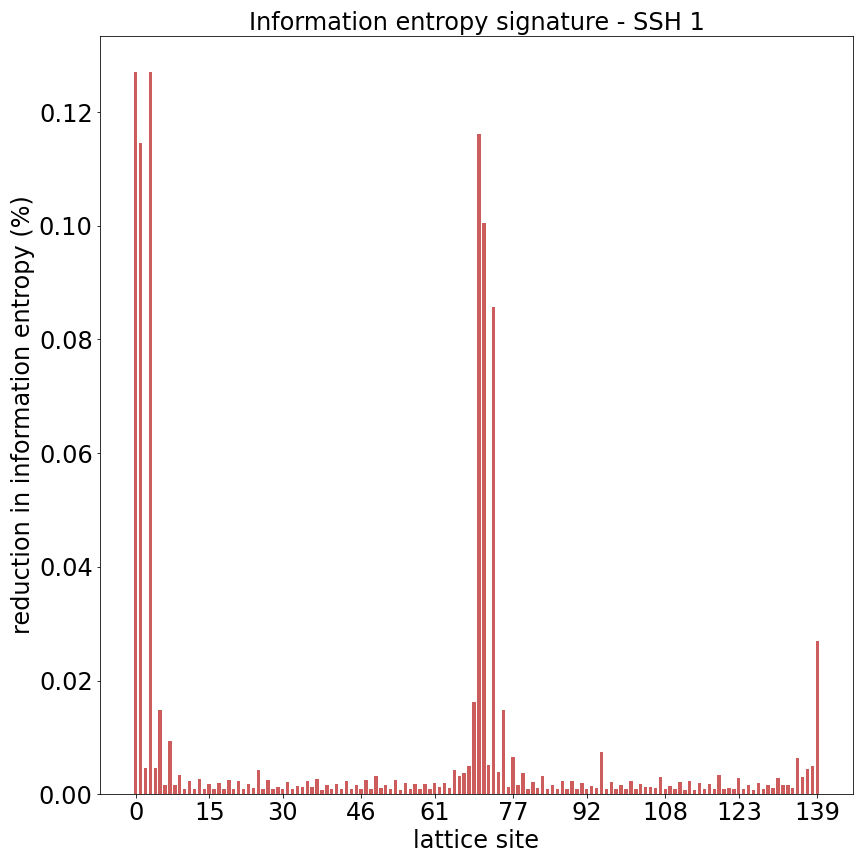
\includegraphics[width=.32\textwidth]{./ssh1/periodic_140_6561/plot_feature_importances.png}}
\subfigure[]{\label{feature_importances_ssh1_180}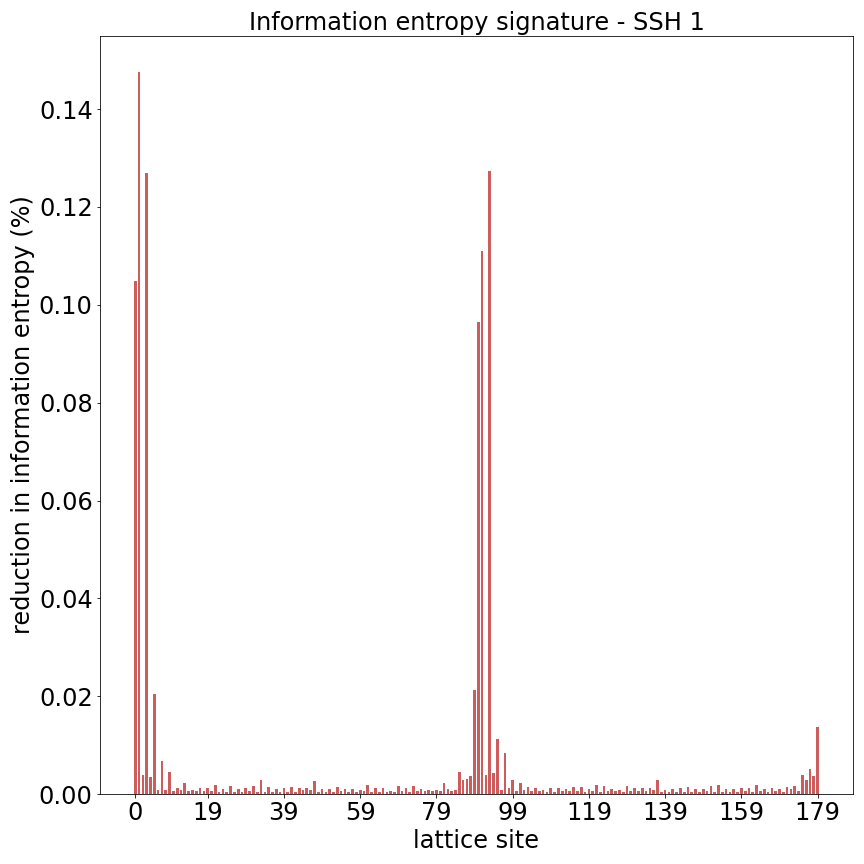
\includegraphics[width=.32\textwidth]{./ssh1/periodic_180_6561/plot_feature_importances.png}}
\subfigure[]{\label{feature_importances_ssh1_220}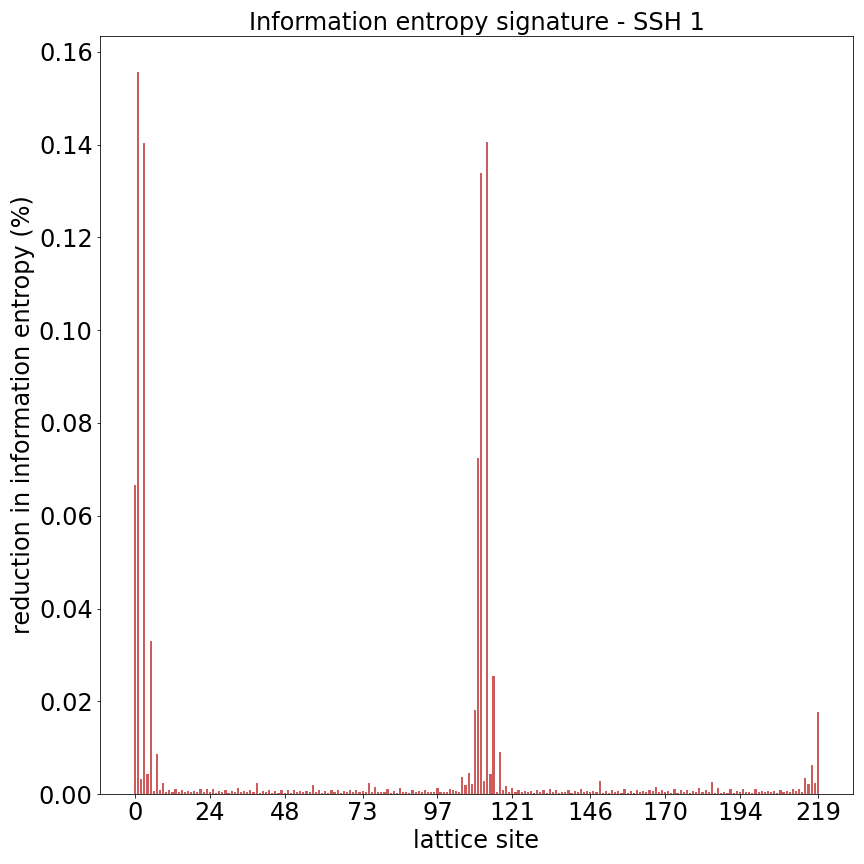
\includegraphics[width=.32\textwidth]{./ssh1/periodic_220_6561/plot_feature_importances.png}}
\caption{Information entropy signatures obtained for experiment 1 with higher lattice sizes. (a) Information entropy signature for 70 unit cells. (b) Information entropy signature for 90 unit cells. (c) Information entropy signature for 110 unit cells.}
\label{feature_importances_ssh1_longer_lattices}
\end{figure}
\begin{figure}
\centering
\subfigure[]{\label{feature_importances_ssh2_140}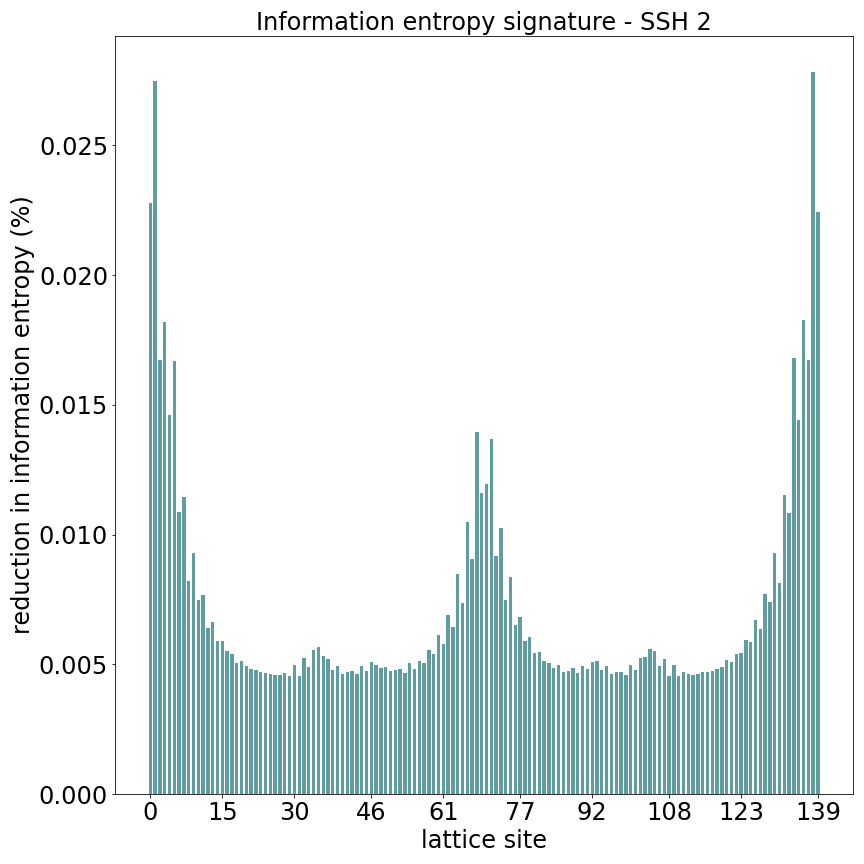
\includegraphics[width=.32\textwidth]{./ssh2/periodic_140_6561/plot_feature_importances.png}}
\subfigure[]{\label{feature_importances_ssh2_180}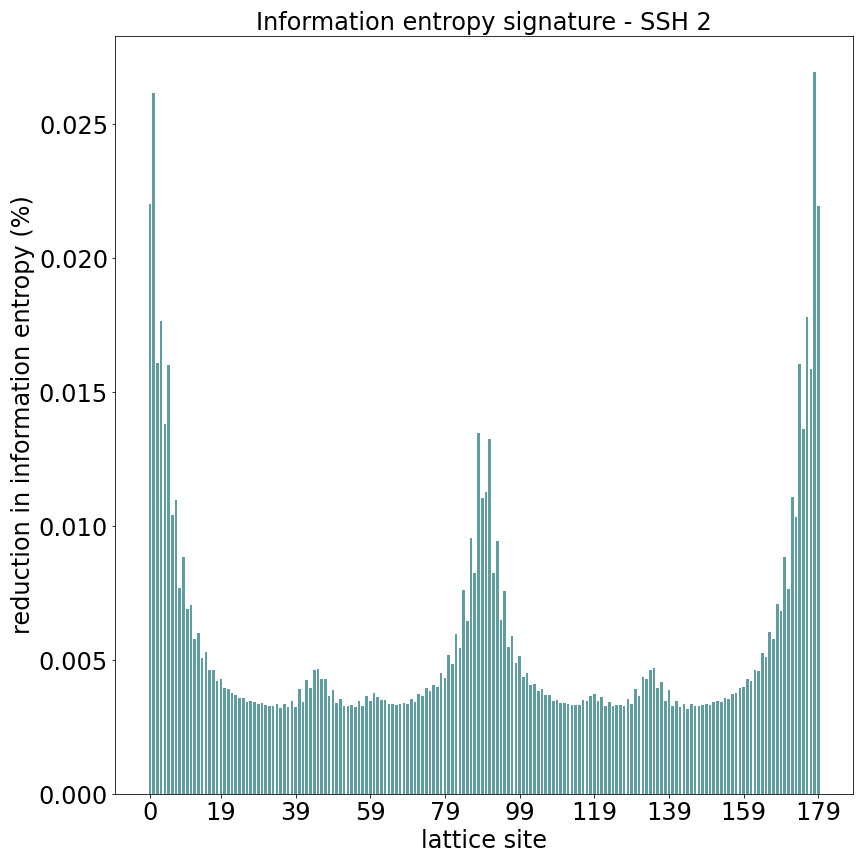
\includegraphics[width=.32\textwidth]{./ssh2/periodic_180_6561/plot_feature_importances.png}}
\subfigure[]{\label{feature_importances_ssh2_220}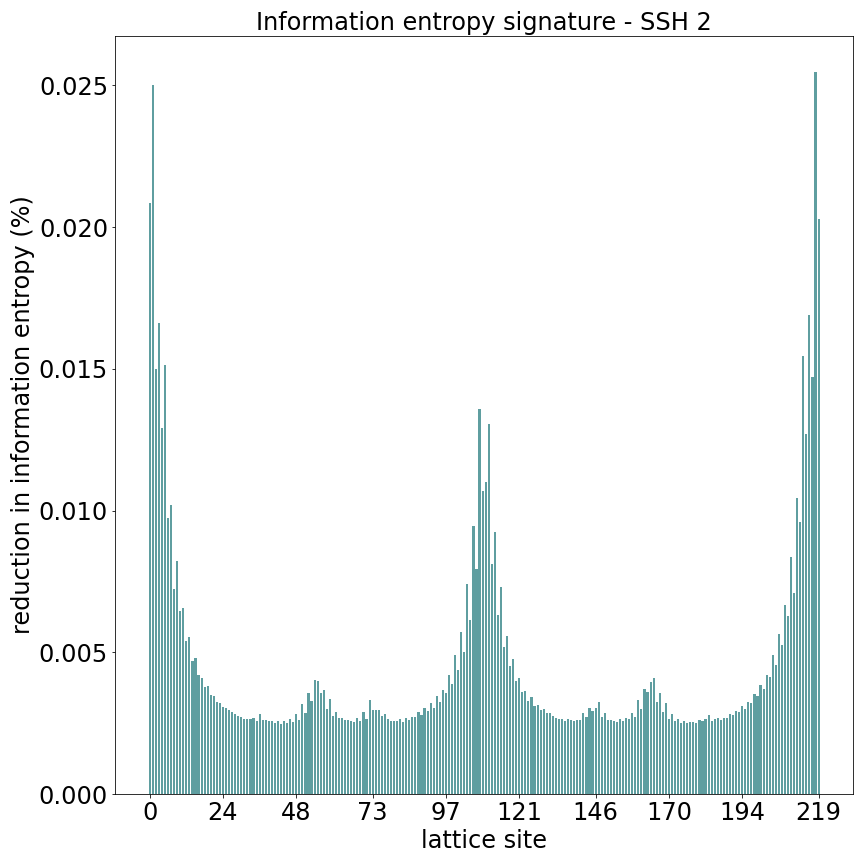
\includegraphics[width=.32\textwidth]{./ssh2/periodic_220_6561/plot_feature_importances.png}}
\caption{Information entropy signatures obtained for experiment 2 with higher lattice sizes. (a) Information entropy signature for 70 unit cells. (b) Information entropy signature for 90 unit cells. (c) Information entropy signature for 110 unit cells.}
\label{feature_importances_ssh2_longer_lattices}
\end{figure}

\begin{figure}
\centering
\subfigure[]{\label{cumulative_entropy_ssh1_140}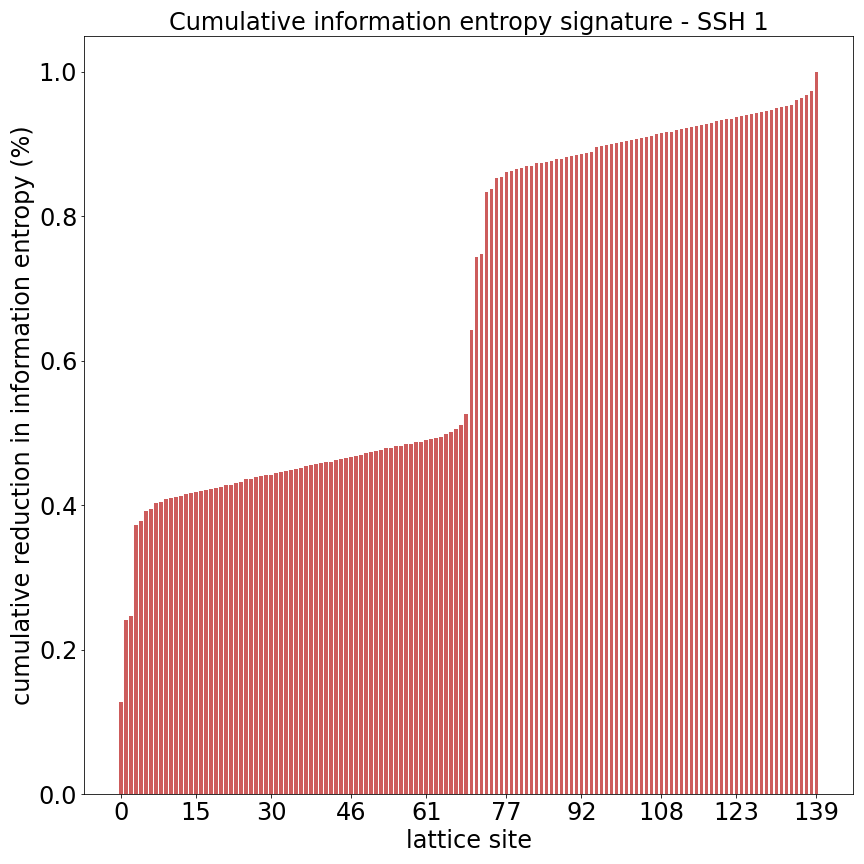
\includegraphics[width=.32\textwidth]{./ssh1/periodic_140_6561/plot_cumulative_feature_importances}}
\subfigure[]{\label{cumulative_entropy_ssh1_180}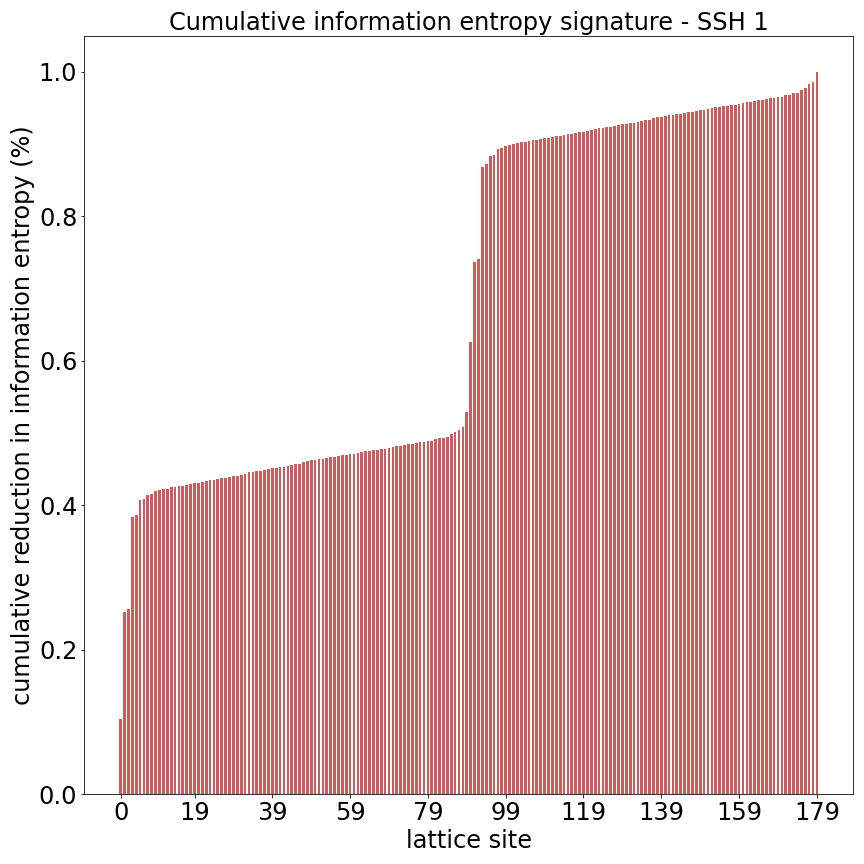
\includegraphics[width=.32\textwidth]{./ssh1/periodic_180_6561/plot_cumulative_feature_importances}}
\subfigure[]{\label{cumulative_entropy_ssh1_220}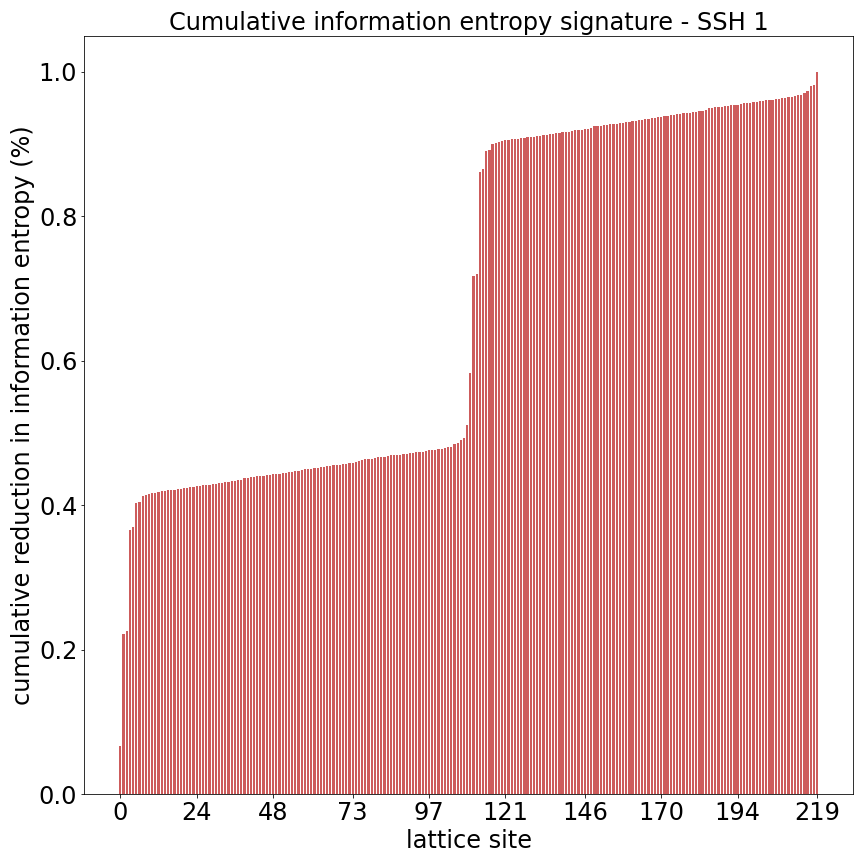
\includegraphics[width=.32\textwidth]{./ssh1/periodic_220_6561/plot_cumulative_feature_importances}}
\caption{Cumulative entropy distributions for higher lattice sizes in experiment 1. (a) Cumulative entropy distribution for 70 unit cells. (b) Cumulative entropy distribution for 90 unit cells. (c) Cumulative entropy distribution for 110 unit cells. The two visible leaps in the cumulative entropy distributions shown above occur at regions corresponding to the lattice sites $S_1$ in the case with 50 unit cells.}
\label{cdf1}
\end{figure}

\begin{figure}
\centering
\subfigure[]{\label{cumulative_entropy_ssh2_140}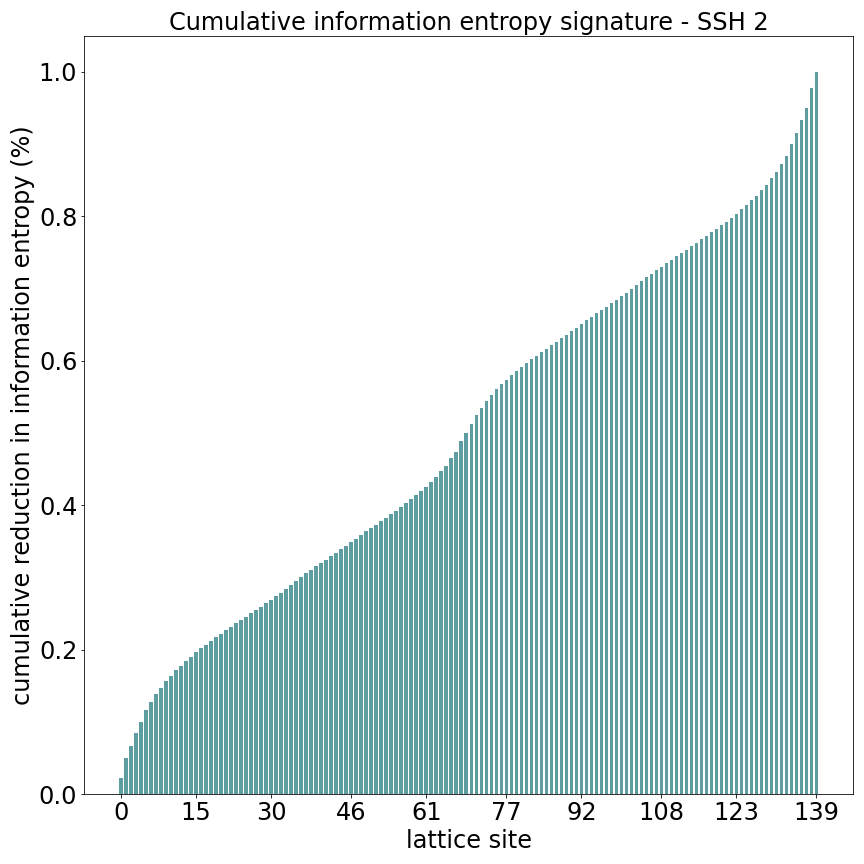
\includegraphics[width=.32\textwidth]{./ssh2/periodic_140_6561/plot_cumulative_feature_importances}}
\subfigure[]{\label{cumulative_entropy_ssh2_180}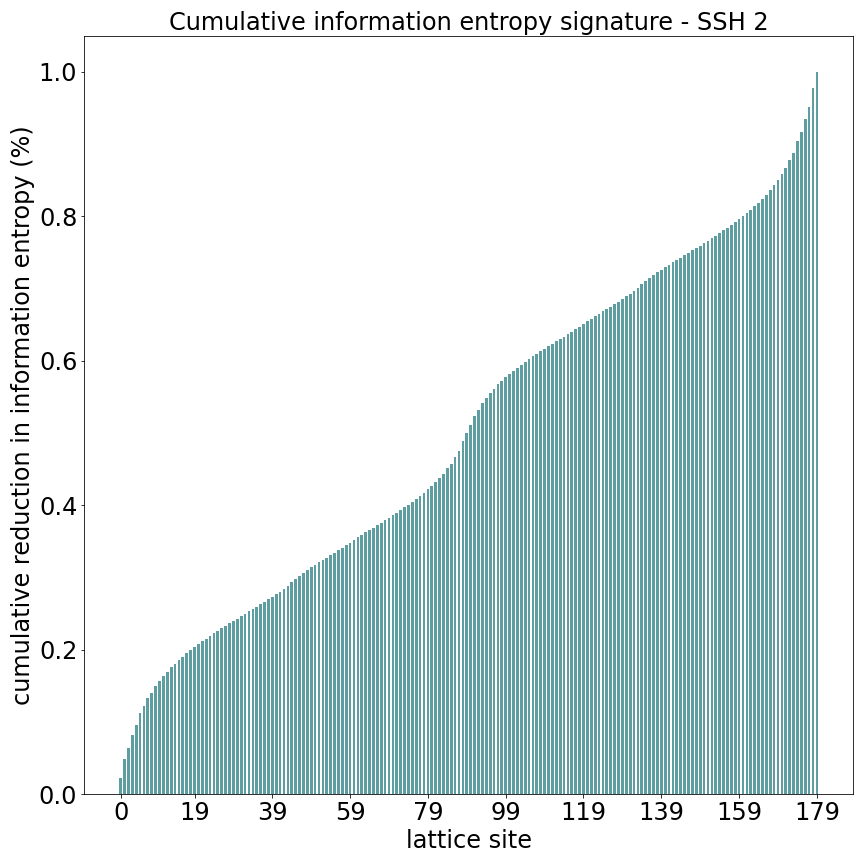
\includegraphics[width=.32\textwidth]{./ssh2/periodic_180_6561/plot_cumulative_feature_importances}}
\subfigure[]{\label{cumulative_entropy_ssh2_220}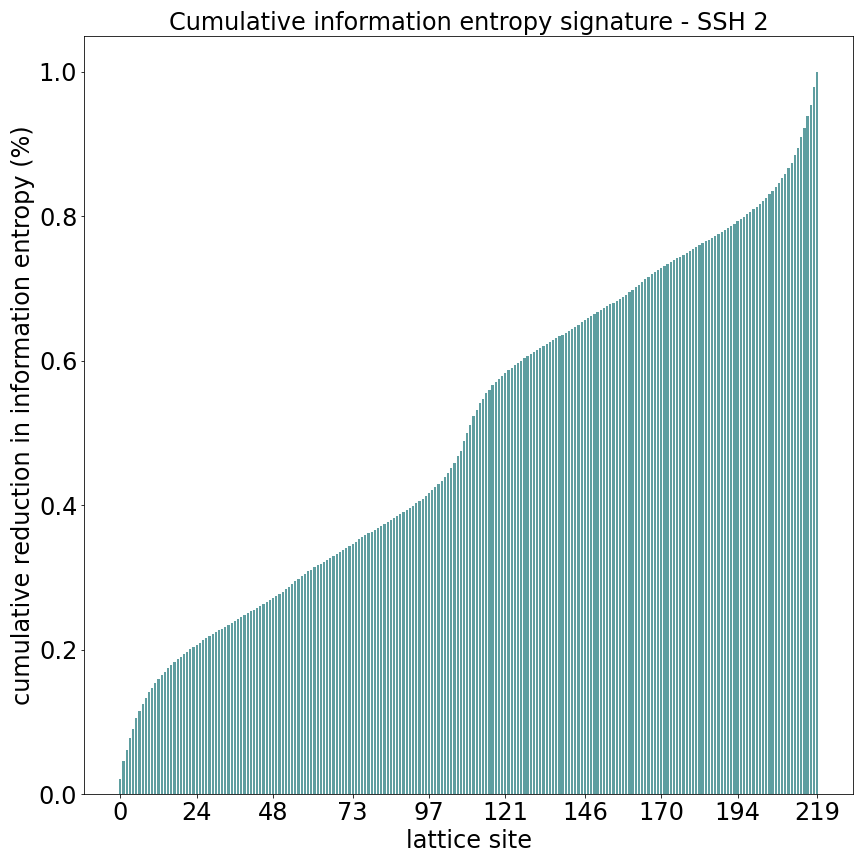
\includegraphics[width=.32\textwidth]{./ssh2/periodic_220_6561/plot_cumulative_feature_importances}}
\caption{Cumulative entropy distributions for higher lattice sizes in experiment 2. (a) Cumulative entropy distributions for 70 unit cells. (b) Cumulative entropy distributions for 90 unit cells. (c) Cumulative entropy distributions for 110 unit cells. Here the leaps in the cumulative entropy distributions are less pronounced than in experiment 1, but still noticeable. The three visible leaps occur at regions corresponding to the lattice sites $S_2$ in the case of 50 unit cells.}
\label{cdf2}
\end{figure}

%\newpage
%\bibliographystylesupp{naturemag-doi}
%\bibliographysupp{supp}

\end{document}







